\begin{refsection}
\chapter{Acúmulo de mutações deletérias em genes que foram alvos de seleção balanceadora de longo prazo em humanos}
%\addcontentsline{toc}{chapter}{Capítulo 2: Accumulation of deleterious mutations in regions under balancing selection}

\fancyfoot[C]{\thepage}
\rhead{Capítulo 2}
\counterwithout{equation}{chapter}
\setcounter{equation}{0}
\counterwithout{figure}{chapter}
\setcounter{figure}{0}
\counterwithout{table}{chapter}
\setcounter{table}{0}
%%%%%%%%%%%%%%%%%%%%%%%%%%%%%%%%%%%%%%%%%%%%%%%%%%%%%%%%%
\section{Considerações Iniciais}

Na última década -- e particularmente nos últimos 5 anos -- diversos trabalhos vêm documentando
a existência de uma parcela relativamente elevada de mutações deletérias em populações humanas. Alguns estudos encontraram 
uma diferença entre a carga genética de populações africanas e não-africanas (\cite{Hodgkinson2013,Lohmueller2008,Lohmueller2014,Henn2016}), ao passo que outros trabalhos vêm contestando tais achados (\cite{Do2015,Simons2014}). Paralelamente, uma série de estudos avaliaram a influência que as \enquote{varreduras seletivas} têm sobre variantes neutras próximas -- reduzindo a diversidade -- e, menos frequentemente, sobre variantes não-neutras -- limitando a eficácia da seleção nos sítios ligados (\cite{Betancourt2002,Chun2011}). Até o momento, nenhum estudo buscou avaliar o impacto que a seleção para a manutenção de um polimorfismo balanceado tem sobre variantes deletérias ligadas (exceto para HLA, \cite{Lenz2016}). Assim, buscamos testar a hipótese de que a seleção balanceadora sobre um sítios aumenta a abundância de alelos deletérios ligados que, na ausência de seleção balanceadora, poderiam ter sido eliminados por seleção purificadora. 

A fim de abordar essa questão, valemo-nos dos genes com assinaturas de seleção balanceadora identificados no Capítulo 1\footnote{Referimo-nos neste Capítulo ao manuscrito (não publicado) do Capítulo 1 como Bitarello et al. (n.d).}. Neste trabalho tive a colaboração de Débora Y.C. Brandt (doutoranda, Universidade da Califórnia, Berkeley) e Jônatas E. César (pós-doutorando, Universidade de São Paulo, IB), além de Diogo Meyer, que orientou o trabalho. D.Y.C.B. organizou os dados do Projeto 1000 Genomas para nossas análises, calculou as frequências alélicas por população e contribuiu com anotações funcionais para os SNPs. J.E.C. desenvolveu \emph{scripts} eficientes para as abordagens de re-amostragem descritas no manuscrito, além de ter feito o pré-processamento dos dados para nossas análises. Eu participei de todas as etapas descritas, fiz o planejamento das análises a serem feitas (juntamente com D.M. e J.E.C.) e redigi o manuscrito, juntamente com D.M., com colaboração e aprovação dos outros co-autores. Todos contribuíram para a discussão dos resultados. Pretendemos submetê-lo para o periódico \emph{Genetics}.

%%%%%%%%%%%%%%%%%%%%%%%%%%%%%%%%%%%%%%%%%%%%%%%%%%%%%%%%%%%%%%%%%%%%%%%%%%%%%%%%%%%%%%%%%%%%%%%%%%%%%%%%%%%%%%%%%%%%%%%%%%%%%%%%%%
\newpage
\begin{otherlanguage}{english}

\begin{center}

\LARGE{Balancing selection drives the accumulation of linked deleterious variation in humans}


\end{center}

\begin{center}
Bárbara Domingues Bitarello\textsuperscript{1}, Jônatas Eduardo César\textsuperscript{1}, Débora Yoshihara Caldeira Brandt\textsuperscript{2}, Diogo Meyer\textsuperscript{1}
\end{center}

\footnotesize{1, Departamento de Genética e Biologia Evolutiva, Universidade de São Paulo, São Paulo, Brazil}

\footnotesize{2, University of California, Berkeley, USA} 
%%%%%%%%%%%%%%%%%%%%%%%%%%%%%%%%%%%%%%%%%%%%%%%%%%%%%%%%%%%%%%%%%%%%%%%%%%%%%%%%%%%%%%%%%%%%%%%%%%%%%%%%%%%%%%%%%%%%%%%%%%%%%%%%%%
%%%%%%%%%%%%%%%%%%%%%%%%%%%%%%%%%%%%%%%%%%%%%%%%%%%%%%%%%%%%%%%%%%%%%%%%%%%%%%%%%%%%%%%%%%%%%%%%%%%%%%%%%%%%%%%%%%%%%%%%%%%%%%%%%%%%%%%%%%%%%%%%%%%%%%%%%%%%%%%%%%%%%%%%%%%%%%%%%%%%%%%%%%%%%%%%%%%%%%%%%%%%%%%%%%%%%%%%%%%%%%%%%%%%%%%%%
%%%%%%%%%%%%%%%%%%%%%%%%%%%%%%%%%%%%%%%%%%%%%%%%%%%%%%%%%%%%%%%%%%%%%%%%%%%%%%%%%%%%%%%%%%%%%%%%%%%%%%%%%%%%%%%%%%%%%%%%%%%%%%%%%%

%
\normalsize
\section{Introduction}
\lettrine[lines=3]{\color{airforceblue}U}{nderstanding} the dynamics and factors that interfere with the efficacy of natural selection is crucial to understanding phenotypes, complex diseases and genome structure in humans (\cite{Brandvain2016}). Mutations \emph{per se} can be neutral, advantageous, slightly deleterious or strongly deleterious and genomic studies have shown that human populations harbour a large number of deleterious mutations (e.g. \cite{Eyre-Walker1999,Kiezun2013}, among several others). 

Using comparative methods, \textcite{Eyre-Walker1999} estimated that about 1.6 new deleterious mutations arise per human individual per generation. %%this sentence came  from Lohmueller, I need to rephrase and add more references so it doesnt look identical. Perhaps it is unnecessary.
Estimates of load carried per individual vary between three to five (\cite{Morton1956}) and as much as 100 lethal equivalents (\cite{Kondrashov1995}) -- i.e, an allele or combination of alleles that if made homozygous would be lethal (\cite{Lohmueller2008}). More recent estimates vary from 300 to 1,200 deleterious mutations per diploid (human) genome (\cite{Fay2011,Lohmueller2008,Sunyaev2001}). %check these estimates. check if this is not too similar to lohmueller.
All of these estimates mostly reflect the assumed mutation rate, but also rely on effective population size, dominance, and the assumption that populations are in equilibrium (\cite{Brandvain2016}). Moreover, the methods used in the determination of what makes a mutation \enquote{deleterious} vary considerably (reviewed in \cite{Henn2015a}). Therefore, it is possible that many analyses on the load of deleterious mutations carry inaccuracies (reviewed in \cite{Brandvain2016}).

Three  processes have a central role in accounting for the abundance and distribution of deleterious mutations in the genome:  mutation, drift, and selection (\cite{Brandvain2016}). Firstly, the balance between influx via mutation and removal via purifying selection results in a dynamic process, where a large number of weakly selected variants can be maintained at low frequencies. Exome and genome-wide studies reporting an enrichment of recent deleterious mutations are strong evidence for this process (\cite{Casals2013,Fu2012,Tennessen2012,Kiezun2013}).

Secondly, features of a population's demographic history can influence the load of deleterious mutations that it carries. The last decade has seen an explosion of studies comparing the genetic load between human populations (\cite{Tishkoff2002,Lohmueller2008,Lohmueller2014,Simons2014,Henn2015a,Henn2016}). \textcite{Lohmueller2008} quantified the number of deleterious mutations per diploid genome in African American (AA) and European Americans (EA) individuals, finding that EA individuals have lower levels of nucleotide heterozygosity for all functional categories analysed, and a higher number of homozygous genotypes for derived alleles in synonymous and nonsynonymous sites and for "possibly damaging" (\cite{Adzhubei2010}) SNPs.

Although the former result is compatible with a rich body of literature documenting decreasing levels of heterozygosity with increasing distance from Africa (e.g.\cite{Tishkoff2002,Henn2015a}), the second observation is not, \emph{a priori}, expected. Moreover, among the SNPs segregating in only one of the two populations, the proportion of nonsynonymous SNPs was found to be significantly higher in EA (\cite{Lohmueller2008}).

This excess of deleterious mutations in European populations was interpreted as a consequence of a recent out-of-Africa bottleneck ($\sim 50,000$ years ago) followed by explosive population growth until the present (\cite{Lohmueller2008}). Although the African population also experienced  growth, it happened further in the past and thus this population would have had enough time to move closer to equilibrium conditions (\cite{Lohmueller2008}). Later findings supported this hypothesis (\cite{Alkan2009,Subramanian2012,Subramanian2016,Hodgkinson2013,Peischl2013,Peischl2015}), while others disputed it (\cite{Do2015,Simons2014}). 

A third factor that can account for the load in our genomes is pleiotropy, which is widespread in the human genome. For example, several studies show that disease alleles are often also positively selected, indicating that a deleterious variant has been pushed to a high frequency due to some other contribution to fitness it displays (e.g. \cite{Corona2010}). %perhaps mention autoimmune diseases associadtes to HLA?

Here, we explore an additional process that can play a role in shaping the load of mutations: the effect of selection on closely linked loci. It is plausible that at least part of the mutational load in humans is due not to demographic factors, but to indirect consequences of selection in adjacent loci (Figure ~\ref{fig:schema}).

%%%%%%%% Figure %%%%%%%%%%%
%%%%%%%% Figure %%%%%%%%%%%
\begin{figure}[ht]
\centering
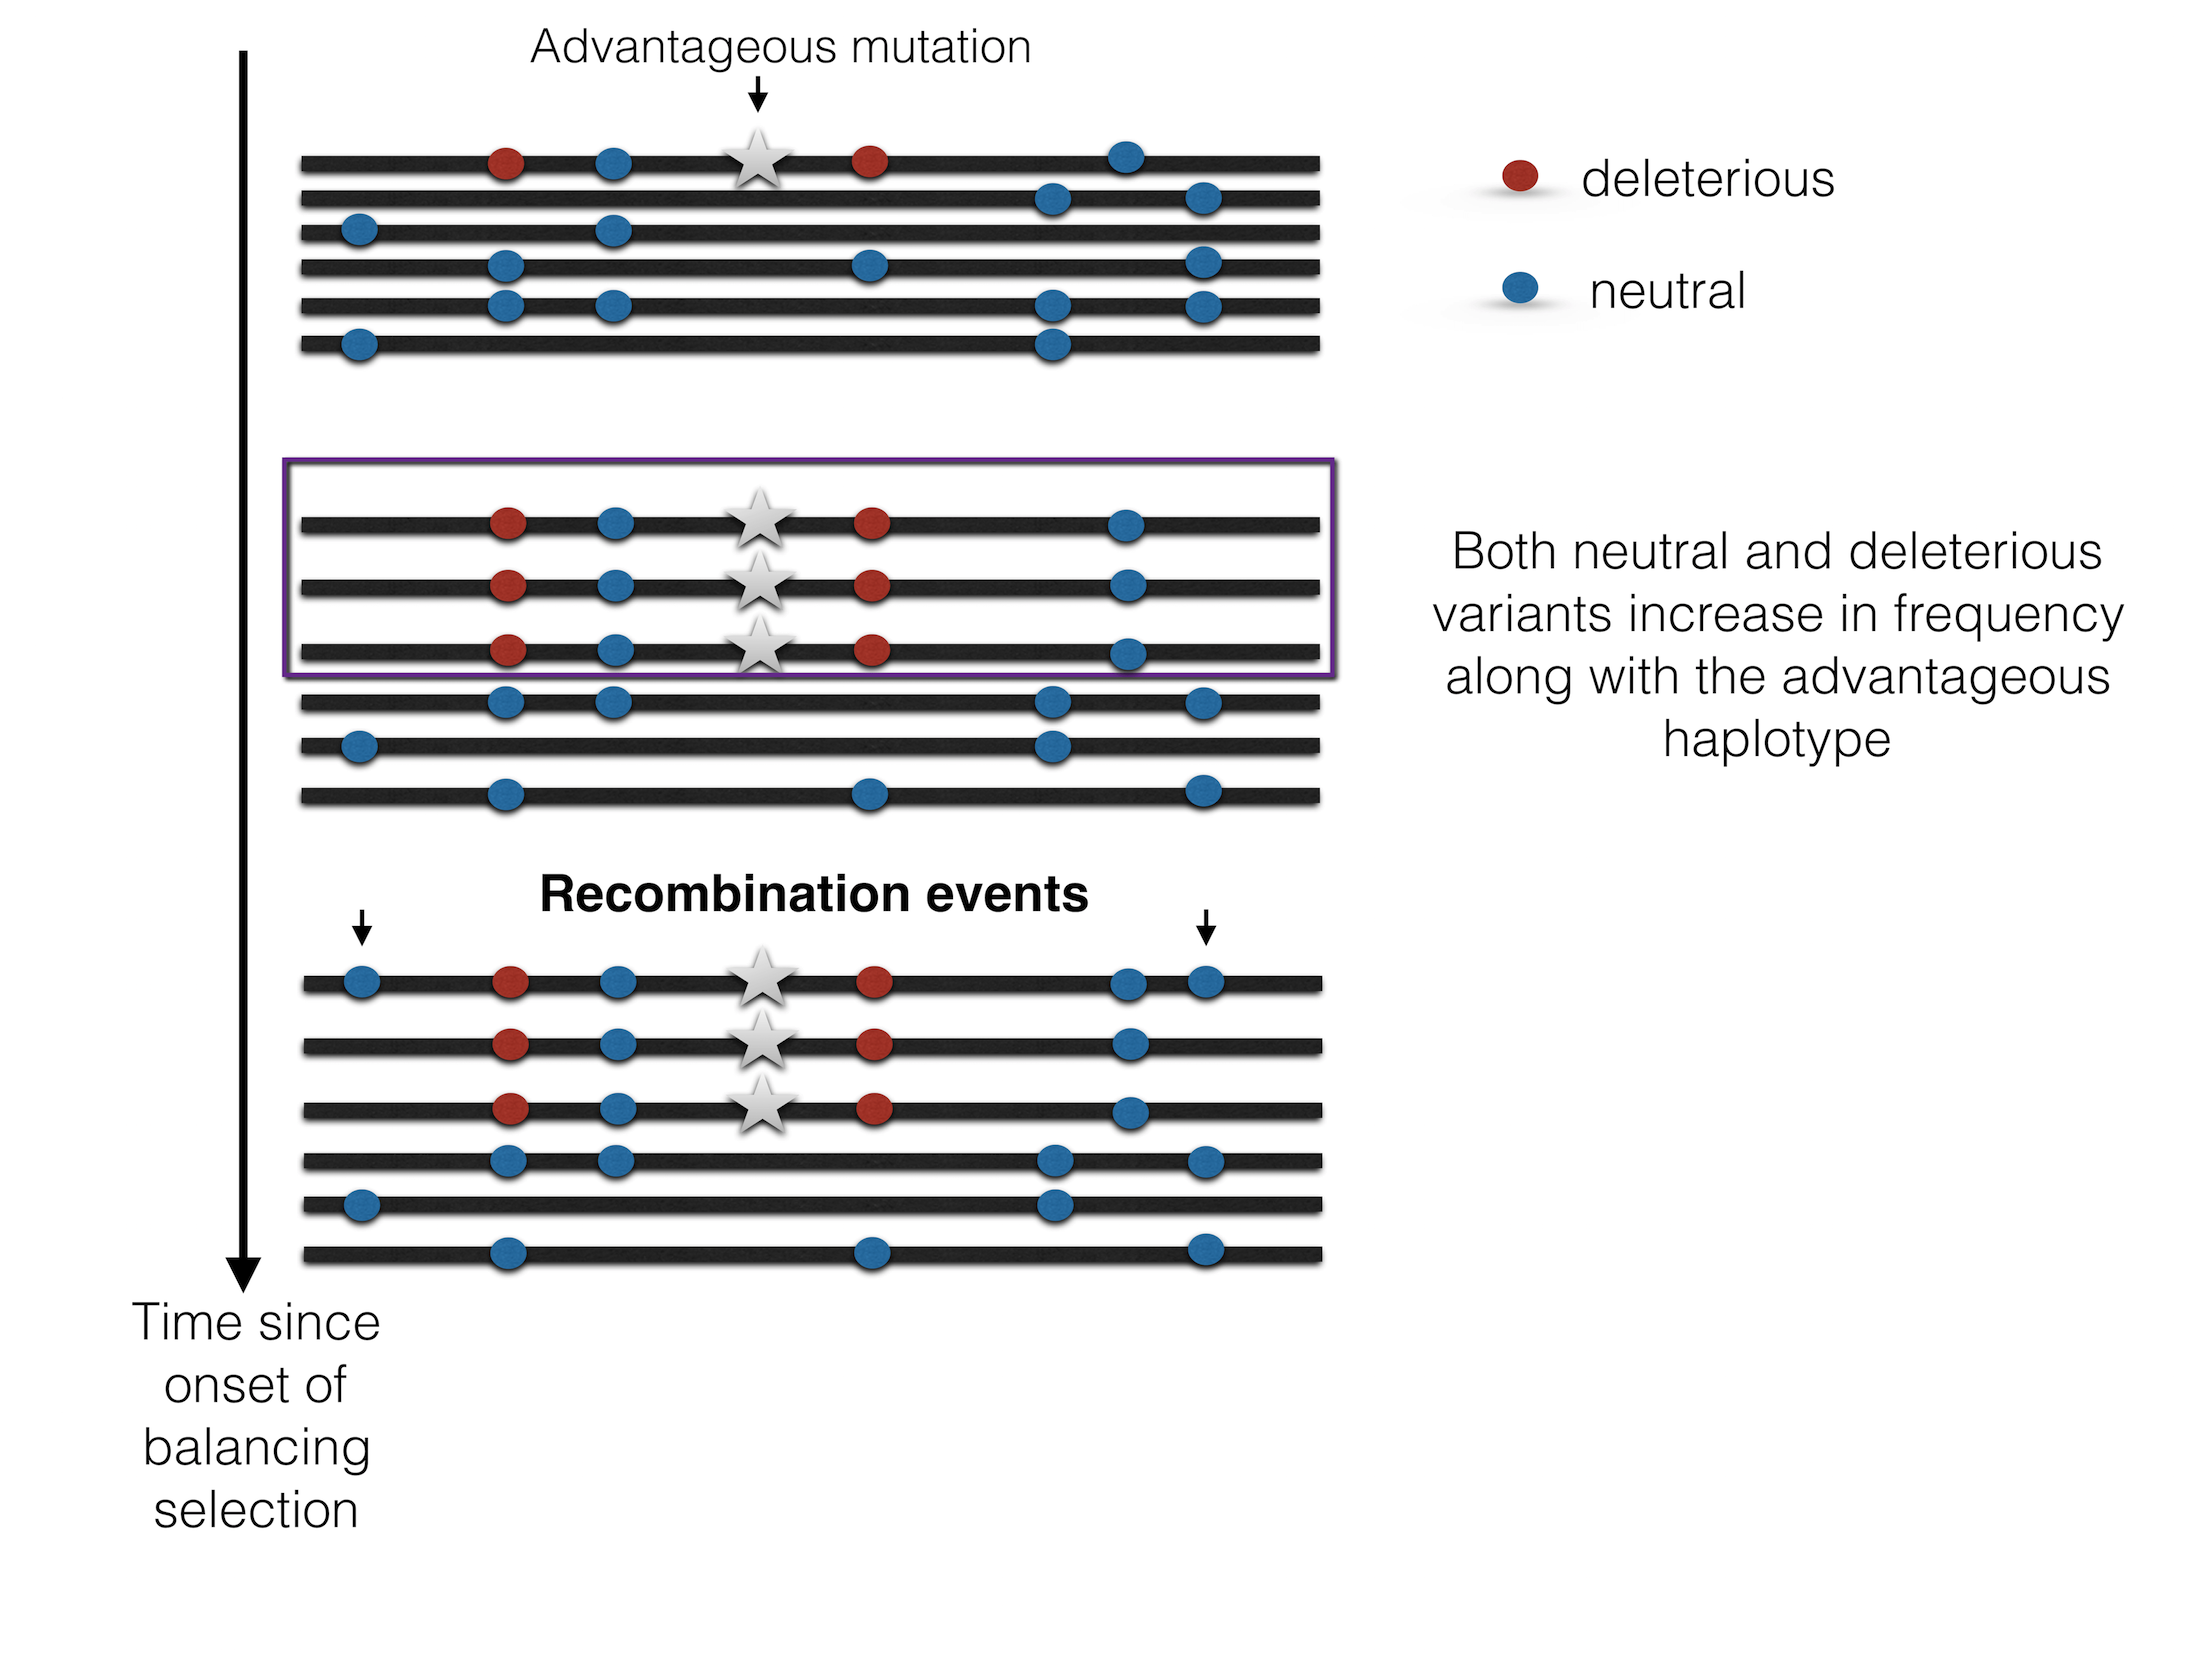
\includegraphics[width=13 cm, keepaspectratio]
{chap3_folder/figures/FIG_1_chap2_tiny.png}
\caption{\textbf{Effect of balanced polymorphism on neighboring sites.} When an advantageous variant appears in a given haplotype, but the site itself is under long-term balancing selection, the advantageous variant increases the frequency of neutral and deleterious variants in linkage. Because two or more haplotypes are maintained, the linked variants are also kept polymorphic. Adapted from \textcite{Charlesworth2006}.}
\label{fig:schema}
\end{figure}
%%%%%%%% Figure %%%%%%%%%%%
%%%%%%%% Figure %%%%%%%%%%%

In this study we take up the task of understanding how  balancing selection in humans has shaped the level of load in adjacent loci. It is well understood how selection -- directional and balancing -- has shaped neutral variation in regions that lie close to sites under either directional or balancing selection (e.g. \cite{Charlesworth2006,Charlesworth2012,Cutter2013,Nielsen2005}, to name a few). Recombination rates and neutral genetic diversity are correlated in several organisms (reviewed in \cite{Charlesworth2012,Cutter2013}) and, when selective sweeps occur, a depletion of neutral diversity is verified around the selected site (\cite{Charlesworth2012,Cutter2013,Nielsen2005}). The extent of this effect is a consequence of both recombination rates and the intensity of selection (\cite{Roux2013,schierup2000effect,Charlesworth1997}).

The effects of directional selection on the accumulation of deleterious mutations are less understood, but have also been addressed (e.g. \cite{Betancourt2002,Chun2011}). Interestingly, studies in \emph{Drosophila} have highlighted that strong purifying (background) selection  hampers the effectiveness of natural selection targeting neighboring sites: near strongly selected sites, there is increased accumulation of deleterious mutations and the effectiveness of selection targeting optimal codon usage is lower (\cite{Betancourt2002}). There is also evidence that directional selection limits the efficacy of purifying selection in neighboring sites in humans (\cite{Chun2011}).


All these findings suggest that there is a complex interaction of different selective forces targeting linked sites and possibly that linkage limits the efficiency of purifying selection in purging deleterious mutations from the genome. In this context, we propose to examine the following question: does balancing selection targeting certain sites in the human genome interfere with the effectiveness of natural selection in nearby sites, as has been observed for strong directional selection? 

From a theoretical point of view, a first expectation is that balancing selection would increase the rate at which deleterious mutations are purged from the genome. This expectation arises because balancing selection \textit{increases} the effective population size ($N_{e}$) of the genomic region under selection \parencite{Charlesworth1997,Roux2013,schierup2000effect}, and increased $N_{e}$ leads to an increase in the efficacy of natural selection. The key to understanding this apparent paradox is to consider that balancing selection often involves the occurrence of partial selective sweeps (i.e., there is an increase in frequency of the favored allele, but not to the point of fixation, followed by other such events, favoring other variants) \parencite{Connallon2013,Albrechtsen2010b}. Such a process enhances diversity, but variation is structured among haplotypes. This process is analogous to the increase in $N_{e}$
for a structured population, where each deme has a small $N_{e}$, but the overall meta-population has a large $N_{e}$ \parencite{Charlesworth1997,Roux2013,schierup2000effect}. Therefore, balancing selection should increase the genetic load in the vicinity of the balanced polymorphism.

To our knowledge, an increase in genetic load in the vicinity of targets of balancing selection has only  very recently been reported for HLA genes (\cite{Mendes2013,Lenz2016}) and has also been suggested for the \enquote{S} loci in \emph{Arabidopsis} and \emph{Solanum}. In \enquote{S} loci it was interpreted in the context of \enquote{sheltered load}, which relies on the assumption that deleterious variants are recessive and are less \enquote{seen} by purifying selection in regions of high heterozygosity (\cite{Stone2004,Roux2013}). 

Therefore, investigating whether an increased proportion of deleterious variants occurs for targets of balancing selection throughout the entire genome has not yet been examined except in the context of HLA genes. We address this question by investigating the levels of accumulation of deleterious mutations in regions surrounding sites previously detected as targets of balancing selection in a powerful genome-wide approach (\cite{Bitarello2016}). Given the broad range of methods that can be used to identify deleterious variants, and the fact that they are frequently not in agreement (reviewed in \cite{Henn2015a}), we opt to use three complementary approaches. Moreover, most deleteriousness measures are negatively correlated with allele frequencies, thus we explicitly consider the effects of allele frequencies in our analyses.

Our expectation, given the theoretical background outlined above, was that regions with evidence for balancing selection would show an enrichment of deleterious variants. In accord with this expectation we found  strong evidence for an increased proportion of nonsynonymous variants within genes with signatures of long-term balancing selection (LTBS), as well as evidence for an increased proportion of deleterious variants.  

%%%%%%%%%%%%%%%%%%%%%%%%%%%%%%%%%%%%%%%%%%%%%%%%%%%%%%%%%%%%%%%%%%%%%%%%%%%%%%%%%%%%%%%%%%%%%%%%%%%%%%%%%%%%%%%%%%%%%%%%%%%%%%%%%%
\section{Methods}

%%%%%%%%%%%%%%%%%%%%%%%%%%%%%%%%%%%%%%
%%%%%%%%%%%%%%%%%%%%%%%%%%%%%%%%%%%%%%
\subsection{Population datasets}
%%%%%%%%%%%%%%%%%%%%%%%%%%%%%%%%%%%%%%
%%%%%%%%%%%%%%%%%%%%%%%%%%%%%%%%%%%%%%

In order to test the hypothesis that sites within genes with evidence for long-term balancing selection (LTBS) show an excess of deleterious variants, we considered all protein-coding SNP positions (nonsynonymous, \emph{N}, and synonymous, \emph{S}) from the 1000 Genomes Phase 3 data (\cite{Auton2015}). We selected SNPs that fall within the  coordinates of genes with signatures of LTBS (\enquote{balanced genes}, see below) or  within the target windows \emph{per se} (\enquote{balanced windows}) (Tables ~\ref{tab:balancedSNPs} and ~\ref{tab:outlierSNPs}).

We used the integrated call sets in VCF format for each chromosome, and calculated reference and alternative allele frequencies per population using VCFtools (\cite{Danecek2011}). We only considered populations from Africa and Europe, and excluded the admixed ones, thus resulting in 10 populations: [Africa: Yoruba in Ibadan, Nigeria (YRI), Luhya in Webuye, Kenya (LWK), Mende in Sierra Leone (MSL), Gambian in Western Division, The Gambia (GWD), Esan in Nigeria (ESN)]; [Europe: Toscani in Italy (TSI), British in England and Scotland (GBR), Iberian populations in Spain (IBS), Finnish in Finland (FIN), Utah residents with Northern and Western European ancestry (CEU)]. We did not include Asian populations because the targets of balancing selection defined by \textcite{Bitarello2016} were only documented for African and European populations. 


%%%%%%%%%%%%%%%%%%%%%%%%%%%%%%%%%%%%%%%%%%%%%%%
%%% Table %%% Table %%% Table %%% Table %%% Table %%% Table 
%%% Table %%% Table %%% Table %%% Table %%% Table %%% Table 
%%% Table %%% Table %%% Table %%% Table %%% Table %%% Table

\begin{sidewaystable}[h]
\centering
\small
\begin{tabular}{@{}cccccccc@{}}
\toprule
 & \multicolumn{7}{c}{Balanced genes} \\ \midrule
\rowcolor[HTML]{9B9B9B} 
{\color[HTML]{000000} POP} & {\color[HTML]{000000} \# sites} & {\color[HTML]{000000} \emph{N}} & {\color[HTML]{000000} \emph{S}} & {\color[HTML]{000000} $P_{del1}$} & {\color[HTML]{000000} $P_{del2}$} & {\color[HTML]{000000} Benign} & {\color[HTML]{000000} Cscore} \\ \cmidrule(r){1-8}
YRI & 3,423(2,961) & \multicolumn{1}{l}{1,871(1,564)} & \multicolumn{1}{l}{1,552(1,397)} & \multicolumn{1}{l}{197(182)} & \multicolumn{1}{l}{262(238)} & \multicolumn{1}{l}{1,300(1,034)} & \multicolumn{1}{l}{10.72(11.36)} \\
LWK & 3,587(3,126) & 1,959(1,654) & 1,628(1,472) & 213(194) & 281(260) & 1,357(1,093) & 10.85(11.52)  \\
MSL & 3,387(2,937) & 1,837(1,543) & 1,550(1,394) & 198(184) & 241(222) & 1,273(1,013) & 10.63(11.26)  \\
GWD & 3,550(3,098) & 1,967(1,668) & 1,583(1,430) & 198(181) & 292(272) & 1,353(1,091) & 10.75(11.35)  \\
ESN & 3,261(2,821) & 1,804(1,517) & 1,457(1,304) & 202(187) & 265(248) & 1,238(984) & 10.91(11.63) \\
TSI & 2,596(2,146) & 1,479(1,181) & 1,117(965) & 175(161) & 230(211) & 997(733) & 10.88(11.82)  \\
GBR & 2,299(1,866) & 1,328(1,043) & 971(823) & 155(140) & 188(173) & 919(664) & 10.69(11.70) \\
FIN & 2,149(1,715) & 1,230(948) & 910(767) & 138(124) & 173(159) & 864(610) & 10.33(11.36) \\
CEU & 2,353(1,925) & 1,334(1,054) & 1,019(871) & 145(132) & 198(183) & 924(672) & 10.66(11.66)  \\
IBS & 2,612(2,153) & 1,507(1,200) & 1,105(953) & 171(155) & 237(216) & 1,034(764) & 10.82(11.71)  \\ \bottomrule
\end{tabular}
\caption{\textbf{Statistics for protein-coding SNPs  within the balanced genes}. Genes under balancing selection were defined by \textcite{Bitarello2016}. Numbers in parentheses refer to the datasets after removal of HLA genes (see Methods). Cscore, average scaled C score for all SNPs in the set (see Methods). $P_{N}$ and $P_{S}$, numbers of nonsynonymous and synonymous sites, respectively. $P_{del1}$, $P_{del2}$, and Benign, numbers of possibly damaging, probably damaging and benign variants (\cite{Adzhubei2010}), respectively.
}
\label{tab:balancedSNPs}
\end{sidewaystable}
%%%%%%%%%%%%%%%%%%%%%%%%%%%%%%%%%%%%%%%%%%%%%%%%%%%%%%%%%%%%%%%%%%%%%%%%%%%%%%%%%%%%%%%%%%%%%%%%%%%%%%%%%%%%%%%%%%%%%%%%%%%%%%%%%%%%%%%%%%%%%%%%%%%%%%%%%%%%%%%%%%

%%%%%%%%%%%%%%%%%%%%%%%%%%%%%%%%%%%%%%%%%%%%%%%%%%%%%%%%%
%%%%%%%%%%%%%%%%%%%%%%%%%%%%%%%%%%%%%%%%%%%%%%%%%%%%%%%%%

\subsection{Targets of balancing selection} 
%%%%%%%%%%%%%%%%%%%%%%%%%%%%%%%%%%%%%%%%%%%%%%%%%%%%%%%%%
%%%%%%%%%%%%%%%%%%%%%%%%%%%%%%%%%%%%%%%%%%%%%%%%%%%%%%%%%
%%%%%%%%%%%%%%%%%%%%%%%%%%%%%%%%%%%%%%%%%%%%%%%%%%%%%%%%%


	The "balanced genes" are those reported by \textcite{Bitarello2016} (see their Table 3) as having the strongest statistically significant signatures of LTBS in humans (213 genes in total). The list of balanced genes was generated by intersecting 3 Kb windows with strong signatures of LTBS with the protein-coding gene annotation from Encode/Ensembl (\cite{Bitarello2016}). Here we test the hypothesis of an enrichment in the proportion of deleterious variants in the balanced genes \emph{per se} (Table ~\ref{tab:balancedSNPs}). 

A more specific definition of the regions under balancing selection would involve the analysis of "balanced windows" (i.e., the queried sub-region of a gene with evidence for balancing selection, according to the method of \textcite{Bitarello2016}. However, this approach generates a dataset which is too restrictive (Table ~\ref{tab:outlierSNPs}), with a number of SNPs that is too small to provide reliable contrasts among regions under balancing selection with respect to the rest of the genome  (with on average 209 protein-coding SNPs per population, after the HLA genes are removed). We therefore chose to restrict our analyses to the balanced genes, for which we have a larger number of SNPs documenting the influence of selection on nearby sites.
% Seu ponto ficaria ainda mais forte se vocÊ reportasse o número de average number of "coding SNPs" per population, e não o total, pois aí daria para ver que para a análise de pn/ps e pdel/pneu o número realmente despenca.
%BDB;esse núemro é N+S, que eu acho que é o que você sugere, exatamente.


%In principle, testing for an enrichment of deleterious variants within the balanced windows would be restricting analyses to relatively narrow regions of the genome, for which there is strong evidence of balancing selection. This is consistent not only with what is expected for long-term balancing selection (\cite{Hudson1988,Charlesworth2006}), but also with human-specific demography, mutation and recombination rates  (\cite{Andres2009,Bitarello2016,Gravel2011,Roux2013}). 
% Eu acho que agora dá para tirar esse parágrafo e ir direto par ao próximo.

%When testing for an enrichment of deleterious variants within the whole gene for which we have evidence for balancing selection, our inquiry extends to a larger region than when focusing on the portion of the gene with evidence for being directly under balancing selection. There is a trade-off involved with these two approaches: window-based analyses contain few SNPs but correspond to regions with extreme deviations from neutrality; gene-based analyses are performed on a greater number of SNPs, but these are on average more distant from the site(s) of selection, and thus may include cases in which the effect of linked selection is weaker. Nevertheless, given that the windows used to detect targets of long-term balancing selection in \cite{Bitarello2016} are narrow (length of 3kb), the  gene-based approach (see below) has the advantage of directly measuring the effect of the  balanced polymorphisms within a gene over its nearby sites -- i.e, the remaining positions of the gene. 

% Eu acho que com a frase que eu propus esse trecho se torna desnecessário, pois já apresntei de cara a ideia de que o número de SNPs restrito sugere a remoção. Essa sugestão elimina um parágrafo inteiro (dois, na vereade), mas acho que ganhamos em clareza. E eu irei acrescentar material em outros lugares, de modo que o texto não corre risco de "encolher demais".
%BDB: ok...vou remover, mas acho que isso talvez não fique claro pra banca.

Our approach consists in a comparison of the number of deleterious SNPs within the genes under balancing selection and the remainder of the genome (which we refer to as providing a set of "control SNPs"). We define control SNPs as those protein-coding SNPs outside all balanced genes. We did not consider the SNPs contained in the sex chromosomes nor in the mitochondrial DNA since there is no information regarding balancing selection signatures for those genes (\cite{Bitarello2016}). More details about the controls are provided below in the "Re-sampling control SNPs" section. %check the name of this section at the end.

%%%%%%%%%%%%%%%%%%%%%%%%%%%%%%%%%%%%%%%%%%%%%%%%%%%%%%%%%%%%%%%%%%%%%%%%%%%%%%%%%

\begin{table}[h]
\centering
\small
\begin{tabular}{@{}cccccccc@{}}
\toprule
 & \multicolumn{7}{c}{Balanced windows} \\ \midrule
\rowcolor[HTML]{9B9B9B} 
{\color[HTML]{000000} POP} & {\color[HTML]{000000} \# sites} & {\color[HTML]{000000} \emph{N}} & {\color[HTML]{000000} \emph{S}} & {\color[HTML]{000000} $P_{del1}$} & {\color[HTML]{000000} $P_{del2}$} & {\color[HTML]{000000} Benign} & {\color[HTML]{000000} Cscore} \\ \cmidrule(r){1-8}
YRI & 635(225) & 401(124) & 234(102) & 23(9) & 30(9) & 333(93) & 7.50(9.26) \\
LWK & 651(236) & 400(122) & 251(114) & 29(12) & 28(8) & 332(9) & 7.34(9.07) \\
MSL & 636(234) & 391(124) & 245(110) & 20(7) & 29(10) & 327(93) & 7.52(9.29) \\
GWD & 652(248) & 406(136) & 246(112) & 29(13) & 35(16) & 328(93) & 7.88(9.91) \\
ESN & 630(235) & 387(125) & 243(110) & 28(13) & 24(8) & 321(91) & 7.46(9.43) \\
TSI & 612(205) & 388(113) & 224(92) & 27(13) & 33(15) & 317(75) & 7.62(9.93) \\
GBR & 561(171) & 361(100) & 200(71) & 24(9) & 28(14) & 302(70) & 7.25(9.31) \\
FIN & 553(166) & 351(91) & 202(75) & 22(8) & 24(10) & 297(65) & 7.02(8.80) \\
CEU & 559(172) & 353(96) & 206(76) & 19(6) & 28(14) & 297(67) & 7.17(9.29) \\
IBS & 607(196) & 384(107) & 223(89) & 26(11) & 33(15) & 314(70) & 7.46(9.58) \\ \bottomrule
\end{tabular}
\caption{\textbf{Statistics for protein-coding SNPs within balanced windows}. Windows are defined in \textcite{Bitarello2016}. Cscore, average scaled C score for all SNPs in the set (see Methods). $P_{N}$ and $P_{S}$, numbers of nonsynonymous and synonymous sites, respectively. $P_{del1}$, $P_{del2}$, and Benign, numbers of possibly damaging, propably damaging and benign variants, respectively (\cite{Adzhubei2010}).
}
\label{tab:outlierSNPs}
\end{table}
%%%%%%%%%%%%%%%%%%%%%%%%%%%%%%%%%%%%%%%%%%%%%%%%%%%%%%%%%
%%%%%%%%%%%%%%%%%%%%%%%%%%%%%%%%%%%%%%%%%%%%%%%%%%%%%%%%%
%%%%%%%%%%%%%%%%%%%%%%%%%%%%%%%%%%%%%%%%%%%%%%%%%%%%%%%%%%%%%%%%%%%%%%%%%%%%%%%%%%%%%%%%%%%%%%%%%%%%%%%%%%%%%%%%%%%%%%%%%%%%%%%%%%%%%%%%%%%%%%%%

%%%%%%%%%%%%%%%%%%%%%%%%%
\subsection{Annotation} 
%%%%%%%%%%%%%%%%%%%%%%%%%

One of the summary statistics used to quantify the genetic load was the CADD (Combined Annotation Dependent Depletion, or simply \enquote{C Score}) described in \textcite{Kircher2014}. Thus, we used the annotation provided in the study of \textcite{Kircher2014}  (available at: \url{http://cadd.gs.washington.edu/download}, accessed in March 2016).

From this annotation file we retrieved the following information: "CHR" (chromosome where the SNP is situated), "POS" (position of SNP in chromosome),  "Consequence" (nonsynonymous, synonymous, 3-prime-UTR, 5-prime-UTR, intronic, non-coding change, canonical splice,stop-gained, stop-lost),  "GeneName" (associated gene name to the SNP position), "AnnoType" (NonCodingTranscript, Transcript, CodingTranscript), "PolyPhenCat" (benign, possibly damaging, probably damaging), and the scaled and raw C scores (\cite{Kircher2014}). 

Because two of our measurements of genetic load (see below) are only applicable to protein-coding sites, we restricted our analyses to these categories. Thus, all quantification of deleterious load was restricted to sites which are protein-coding (i.e., \emph{N} or \emph{S}) (Tables ~\ref{tab:balancedSNPs} and ~\ref{tab:outlierSNPs}). For the step where we identified the specific SNPs with highest heterozygosity for each gene (and which is/are the putative target(s) of balancing selection, see below) we used the complete set of sites within the gene, since it is plausible that sites which are not protein-coding are under balancing selection. 

Given that the effect of balancing selection on the load of nearby regions is also expected to affect sites which are functional but not protein-coding, our approach could theoretically be extended to this class of sites (for example, using a measure of deleteriousness such as the C score, which is applicable to these sites as well). However, in the present study we opted to restrict our analyses to variants that affect protein-coding sequences. We justify this based on the fact that assignment of deleteriousness at these sites can be performed by estimating the ratio of nonsynonymous to synonymous polymorphisms, a measure which is based exclusively on the nature of the variants, with no direct influence of allele frequencies and phylogenetic conservation. 

\afterpage{\FloatBarrier}
%%%%%%%%%%%%%%%%%%%%%%%%%%%%%%%%%%%%%%%%%%%%%%%%%%%%%%%%%%%%%%
%%%%%%%%%%%%%%%%%%%%%%%%%%%%%%%%%%%%%%%%%%%%%%%%%%%%%%%%%%%%%%
\subsection{Quantifying genetic load} 
%%%%%%%%%%%%%%%%%%%%%%%%%%%%%%%%%%%%%%%%%%%%%%%%%%%%%%%%%%%%%%
%%%%%%%%%%%%%%%%%%%%%%%%%%%%%%%%%%%%%%%%%%%%%%%%%%%%%%%%%%%%%%
All protein-coding SNPs from the set of balanced SNPs (Table ~\ref{tab:balancedSNPs}) were jointly considered when calculating the statistics below, i.e, a single estimate of load was made for the entire set of genes with evidence for balancing selection. This avoids the difficulty in obtaining reliable estimates when computing load for individual genes, since these often have a small number of SNPs. For controls, the same approach was adopted for each re-sampled set of SNPs (details below). 

%%%%%%%%%%%%%%%%%%%%%%%%%%%%%%%%%%%%%%%%%%%%%%%%%%%%%%%%%%%%%%%%%%%%%%
\subsubsection{Ratio of nonsynononymous to synonymous polymorphisms}
%%%%%%%%%%%%%%%%%%%%%%%%%%%%%%%%%%%%%%%%%%%%%%%%%%%%%%%%%%%%%%%%%%%%%%

We calculated the ratio of the number of nonsynonymous ($P_{N}$) to synonymous polymorphisms ($P_{S}$) for each set of SNPs (from balanced genes and controls):

\begin{equation}
P_{N}/P_{S}=\frac{P_{N}}{P_{S}}
\end{equation} 

This ratio provides a  measure of of the proportion of  deleterious mutations, assuming that a large proportion (\cite{Eyre-Walker1999,Subramanian2012}) of nonsynonymous mutations are either strongly or mildly deleterious. However, because nonsynonymous variants include those that are adaptive or neutral, we also considered alternative statistics which quantify genetic load.

%%%%%%%%%%%%%%%%%%%%%%%%%%%%%%%%%%%%%%%%%%%%%%%%%%%%%%%%%%%%%%%
\subsubsection{Ratio of damaging to synonymous polymorphisms}
%%%%%%%%%%%%%%%%%%%%%%%%%%%%%%%%%%%%%%%%%%%%%%%%%%%%%%%%%%%%%%%

To estimate the number of damaging alleles in the \enquote{balanced} and control sets of SNPs, we used the PolyPhen-2 (\cite{Adzhubei2010}) annotation provided in \textcite{Kircher2014}. PolyPhen-2 classifies nonsynonymous variants as either benign, possibly damaging ($P_{del1}$) and probably damaging ($P_{del2}$). We thus defined the ratio of damaging to synonymous SNPs (\cite{Lohmueller2008}) as:

\begin{equation}
P_{del}/P_{S}=\frac{P_{del1}+P_{del2}}{P_{S}}
\end{equation}

This estimate quantifies the proportion of SNPs most likely to be deleterious. PolyPhen-2 is a protein-level metric which is, by definition, restricted to nonsynoymous sites. Moreover, several nonsynonymous SNPs ($\sim 20$\% in the 1000 Genomes dataset) lack PolyPhen-2 annotation, so the $P_{del}/P_{S}$ statistic was calculated based on a smaller set of SNPs than the $P_{N}/P_{S}$ (Tables ~\ref{tab:balancedSNPs} and ~\ref{tab:outlierSNPs}) and has higher variance. %not shown.

%%%%%%%%%%%%%%%%%%%%%%%%%%%
\subsubsection{CADD (C score)}
%%%%%%%%%%%%%%%%%%%%%%%%%%%


 The C score was provided by the CADD tool (\cite{Kircher2014}).  The C score is a composite measure using information from more than 60 different such methods to quantify the effects of a mutation and has been shown to differentiate levels of deleteriousness among groups of SNPs (\cite{Kircher2014}). 
As argued by \textcite{Kircher2014}, protein-level metrics such as PolyPhen-2 (\cite{Adzhubei2010}) are the best performing individual annotations (\cite{Kircher2014}), but are restricted to nonsynonymous variants, whereas conservation scores such as GERP++ (\cite{Davydov2010}) cannot distinguish between nonsynonymous and stop-loss variants at a given position.%iamnot sure what this means.
% stop-loss é sabidamente muito mais deletéria pois trunca completamente a proteína, assim como as stop-gain. Mas a classificação simples do polyphen não pega isso. Aliás, é por isso que o paper do Lenz tem gráficos separados para pdel e mutações que geram stop codons.
%BDB: eu entendo, mas não sei sobre o GERP++, e vou precisar estudar isso caso a banca pergunte.
 

We used both the scaled and the raw C scores provided for the 1000G phase 3 SNPs. The scaled C scores range from 1-99 (higher values indicating higher deleteriousness potential). Although counting the number of SNPs above a certain threshold could be used as a strategy, we used the approach of comparing distributions of C scores between groups in order to increase power (\cite{Kircher2014}). Throughout the discussion, when C scores are presented they refer to the average C score of all $N+S$ SNPs contained in a given set of SNPs (balanced or control). We restricted the analyses to these sites  so as to make the results comparable to those of the two other metrics for measuring deleteriousness. 


%%%%%%%%%%%%%%%%
\begin{equation}
Cscore=\frac{\sum\limits_{i=1}^n(C_{N_{i}})+\sum\limits_{i=1}^n(C_{S_{i}})}
{N+S}
\end{equation}
%%%%%%%%%%%%%%%%

, where $n$ is the total number of SNPs in the set of SNPs,  $C_{N_{i}}$ and $C_{S_{i}}$ are the C scores for \emph{N} and \emph{S} SNPs contained in the set of SNPs. The overall C score used in our analyses is thus an average of the C scores of all $N+S$ SNPs contained within the \enquote{balanced} and control sets of SNPs.

Scaled C scores are very useful for identifying a top ranked SNP and easier to interpret, but raw C scores  offer superior resolution for comparison of distributions of scores between groups of variants (\cite{Kircher2014}). Thus, we also compared the distribution of raw C scores for SNPs within balanced genes to those of the re-sampled sets of controls, and performed a one-tailed Mann-Whitney U-test (the alternative hypothesis being that SNPs from balanced genes have higher raw C scores) to compare the balanced SNPs' distribution to each control replicate (significance threshold 5\%).

%%%%%%%%%%%%%%%%%%%%%%%%%%%%%%%%%%%%%%%%%%%%%%%%%%%%%%%%%%%%%%%%%%%%%%%%%%%%%%%%%%
\subsection{Re-sampling control SNPs} 

To test the hypothesis that balanced genes are enriched for deleterious SNPs, we compared the three statistics that measure deleteriousness between the SNPs contained within the genes under balancing selection and a random sample with the same number of SNPs, but chosen from genes with no evidence for balancing selection (controls) (Table ~\ref{tab:balancedSNPs}). We use the distributions of control SNPs to obtain an empirical \emph{p}-value for the SNPs from balanced genes, defined by the fraction of re-sampled distributions with deleteriousness statistics which are more extreme (i.e, higher) than those of the SNPs from the balanced genes.

Previous studies have shown, and we confirm here (see Results) that there is a strong correlation between allele frequency and the probability of a variant being annotated as deleterious (see Results). Because genes/regions under balancing selection are enriched for SNPs at intermediate frequencies (i.e. higher heterozygosities), this effect will itself result in a marked difference between measures of load for balanced genes and the genomic background. In order to control for this effect and guarantee that differences in load are attributable specifically to the effects of linked selection, we compared the proportion of deleterious variants in balanced genes/windows to those of the control sets of SNPs after matching the control SNPs to the frequencies of those in the \enquote{balanced} set. Next we describe the procedure used to re-sample a set of SNPs while controlling for frequency.

Once the protein-coding SNPs from balanced genes had been selected, we followed a similar approach as the one adopted by \textcite{Subramanian2016}: (1) we took the MAF (minor allele frequency) of each protein-coding SNP; (2)  we calculated the log (base 10) of the MAF (logMAF), because in humans the MAF follows an exponential distribution, i.e, a huge proportion of alleles have very low MAF (e.g. \cite{Abecasis2012,Subramanian2016}); (3) we  divided the SNPs into bins according to the logMAF (in our case, we used 9 bins ranging from logMAF={-0.24, 0.1} with a 0.25 interval, encompassing a MAF range of 0.00398-0.5). Given that we did not expect balancing selection to favour derived or ancestral variants preferentially (\cite{Bitarello2016}), using the MAF is appropriate and does not require further filtering of data in order to infer ancestral and derived states. Importantly, once the set of SNPs from balanced genes were divided into bins of logMAF, we were able to quantify the relative contribution of SNPs to each bin, thus allowing the re-sampled sets of SNPs to match the site-frequency spectrum (SFS) of the SNPs observed in balanced genes. We re-sampled from the control SNPs a set following the proportions of each logMAF bin and the total number of SNPs within the set of target genes (Table ~\ref{tab:balancedSNPs}).

This re-sampling schema was designed to account for the fact that all of the genetic load measurements adopted here correlate negatively with allelic frequency (see Results) and that there is an enrichment of intermediate-frequency alleles among the balanced genes (\cite{Bitarello2016}). Each SNP was sampled independently of its location, provided that it was protein-coding, autosomal and matched the logMAF proportions calculated based on the balanced genes. This means that each control set  had the same number of protein-coding SNPs as the balanced genes' set and a similar SFS (Table ~\ref{tab:balancedSNPs}), but those SNPs were not necessarily attributed to the same number of genes as those for the balanced genes.

%TO DO: supplement for chap 1 with the outleir windows? (if I have time).

%%%%%%%%%%%%%%%%%%%%%%%%%%%%%%%%%%%%%%%%%%%%%%%%%%%%%%%%%%%%%%%%%%%%%%%%%
\subsubsection{Excluding adaptively maintained SNPs from load estimates}
%%%%%%%%%%%%%%%%%%%%%%%%%%%%%%%%%%%%%%%%%%%%%%%%%%%%%%%%%%%%%%%%%%%%%%%%%

	Our goal is to test the hypothesis that SNPs within genes under balancing selection have a higher proportion of deleterious variants than expected for a set of control SNPs. However, an excess of deleterious or functional variation could be an outcome of the direct effects of balancing selection. For example, the unusually high proportion of nonsynonymous polymorphism in HLA genes is a consequence of balancing selection directly on functional sites, and not of deleterious variants accumulating as a byproduct of selection on a specific site (e.g. \cite{Hughes1988,Bitarello2015}).
    
    In order to separate the direct  effects of balancing selection from those due to hitch-hiking, we also calculated the genetic load measurements after excluding the sites which are the strongest candidates for balancing selection (thus justifying the assumption that the remainder of the highly polymorphic variants are present due to linkage with this selected variant). This approach relies on the assumption that one or at most one or a few sites are the targets of balancing selection within each gene. 
 
% Think more on how to justify the exclusion of a single site. Is there something in the Leffler paper that indirectly suggests that the shared hahplotypes arise due to selection at single sites? For the paper, I can envisage the figure you produced having 3 or 4 points per population, one with all SNPs, the next after removal of the top candidate, etc.
%BDB: yes, Leffler considers a storng signature when she has two balanced polymorphisms within a given ~4 kb window. This length was derived assuming human paramters AND that there is a balanced polymorphism at ONE SINGLE SITE. She says in the suppl that "if there is more than one site under balancing selection in a region, and in particualr,if multiple sites interact epistatically, then the ancestral segment could be substantially longer."


For each balanced gene, the putatively selected SNPs were identified by locating within the outlier window with evidence for balancing selection (as reported in \cite{Bitarello2016}) the site with the highest heterozygosity. This SNP was then excluded from the  set of SNPs for the balanced genes. When a balanced gene had more than one balanced window, we chose the one with the most extreme signature of LTBS (\cite{Bitarello2016}). 

Heterozygosity was calculated as follows:

\begin{equation}
H_{i}^{*}=2 \cdot [MAF \cdot (1-MAF)]
\end{equation}

, where $i$ is each SNP position and MAF is the minor allele frequency for that position. For this exclusion step, all coding SNPs were considered, not only \emph{N} and \emph{S}, and most of the excluded SNPs were intronic ($\sim 90$\% per population, Table ~\ref{tab:Hremove}). When the most extreme heterozygosity in a gene was shared by multiple SNPs, all were removed. The average number of SNPs removed per gene, across all populations, was 3.8 SNPs. Also, few genes had one or more \emph{N} or \emph{S} SNPs removed by this filter (average 14 genes out of 213, per population). Overall 71 unique (29 \emph{N} and 42 \emph{S}) SNPs were removed across all populations (average 11 N and 34 S per population, Table ~\ref{tab:Hremove}). 



%%%%%%%%%%%%%%%%%%%%%%%
%%%%%%%%%%%%%%%%%%%%%%%
\begin{table}[ht]
\centering
\small
\begin{tabular}{@{}cccccccl@{}}
\toprule
\rowcolor[HTML]{C0C0C0} 
POP & All & Intron & \emph{N} & \emph{S} & 3'UTR & 5'UTR & Splice \\ \midrule
YRI & 762 & 681 & 18 & 19 & 39 & 4 & 1 \\
LWK & 663 & 599 & 8 & 9 & 41 & 5 & 1 \\
MSL & 664 & 599 & 15 & 13 & 33 & 4 & 0 \\
GWD & 693 & 633 & 12 & 14 & 28 & 5 & 1 \\
ESN & 692 & 621 & 16 & 19 & 32 & 3 & 1 \\
TSI & 763 & 704 & 8 & 16 & 33 & 2 & 0 \\
GBR & 841 & 761 & 13 & 15 & 46 & 4 & 2 \\
FIN & 740 & 669 & 8 & 14 & 43 & 6 & 0 \\
CEU & 754 & 700 & 5 & 15 & 33 & 1 & 0 \\
IBS & 715 & 670 & 12 & 12 & 14 & 7 & 0 \\ \bottomrule
\end{tabular}
\caption{\textbf{Classes of SNPs with the highest heterozygosity(ies) per gene} For each gene, the SNP(s) with the highest heterozygosity(ies) were removed (All). Only SNPs contained within the outlier windows (\cite{Bitarello2016}) of those genes were considered. Splice, splice-site position, 3' and 5' UTR, 3 and 5 prime UTR regions, \emph{N}, \emph{S}, Intron, nonsynonymou, synonymous and intronic sites.
}
\label{tab:Hremove}
\end{table}
%%%%%%%%%%%%%%%%%%%%%%%
%%%%%%%%%%%%%%%%%%%%%%%

Given that the assumption that a balanced gene/window has one or a few sites which is/are the actual target(s) of selection is not reasonable for the HLA genes -- where several sites are targets of balancing selection (\cite{Hughes1988,Bitarello2015}) -- we performed our analyses under two scenarios: either keeping the HLA genes or removing them. For these analyses we removed the following HLA genes, which have prior strong evidence for long-term balancing selection and are included among the outlier genes in \textcite{Bitarello2016}: \emph{HLA-A},\emph{HLA-B}, \emph{HLA-C}, \emph{HLA-DRB1}, \emph{HLA-DRB5}, \emph{HLA-DPA1}, \emph{HLA-DPA2}, \emph{HLA-DPB1}, \emph{HLA-DPB2}, \emph{HLA-DQB1}, \emph{HLA-DQB2}, \emph{HLA-DQA1}, \emph{HLA-DQA2}. Their removal changes the proportion of target SNPs that fall into each bin of logMAF, with the SFS becoming less enriched for intermediate frequency variants. 

All analyses and figures were generated in R (\cite{RDevelopmentCoreTeam2009}) and scripts are available: calculation of allele frequencies per population for 1000 Genomes Phase 3 data (\url{https://github.com/deboraycb/1000Gstats_inR/}); load analyses, re-sampling and all figures (\url{https://github.com/ bbitarello/deleterious_mutations}, access can be provided upon request).

%%%%%%%%%%%%%%%%%%%%%%%%%%%%%%%%%%%%%%%%%%%%%%%%%%%%%%%
%%%%%%%%%%%%%%%%%%%%%%%%%%%%%%%%%%%%%%%%%%%%%%%%%%%%%%%
%%%%%%%%%%%%%%%%%%%%%%%%%%%%%%%%%%%%%%%%%%%%%%%%%%%%%%%
%%%%%%%%%%%%%%%%%%%%%%%%%%%%%%%%%%%%%%%%%%%%%%%%%%%%%%%
%%%%%%%%%%%%%%%%%%%%%%%%%%%%%%%%%%%%%%%%%%%%%%%%%%%%%%%
%%%%%%%%%%%%%%%%%%%%%%%%%%%%%%%%%%%%%%%%%%%%%%%%%%%%%%%
%%%%%%%%%%%%%%%%%%%%%%%%%%%%%%%%%%%%%%%%%%%%%%%%%%%%%%%
%%%%%%%%%%%%%%%%%%%%%%%%%%%%%%%%%%%%%%%%%%%%%%%%%%%%%%%
%%%%%%%%%%%%%%%%%%%%%%%%%%%%%%%%%%%%%%%%%%%%%%%%%%%%%%%
%%%%%%%%%%%%%%%%%%%%%%%%%%%%%%%%%%%%%%%%%%%%%%%%%%%%%%%
%%%%%%%%%%%%%%%%%%%%%%%%%%%%%%%%%%%%%%%%%%%%%%%%%%%%%%%
%%%%%%%%%%%%%%%%%%%%%%%%%%%%%%%%%%%%%%%%%%%%%%%%%%%%%%%
\section{Results}
%%%%%%%%%%%%%%%%%%%%%%%%%%%%%%%%%%%%%%%%%%%%%%%%%%%%%%%%%%%%
\subsection{The site frequency spectrum of balanced genes}
%%%%%%%%%%%%%%%%%%%%%%%%%%%%%%%%%%%%%%%%%%%%%%%%%%%%%%%%%%%%

Here, we consider as "balanced genes" the set described as having the strongest signatures of LTBS in \textcite{Bitarello2016}. Balancing selection shifts the SFS towards intermediate frequencies (\cite{Andres2009,Bitarello2016}). Although the selected sites may only comprise a subset of the entire locus, balancing selection changes levels of polymorphism at adjacent sites (neutral and non-neutral), thus generating a signature that allows selected genes to be detected (\cite{Bitarello2016}). It is entirely plausible, and likely, that only portions of those genes are the targets of balancing selection, and this provided us with an appropriate dataset that has the putative site(s) that were selected and their immediate vicinities, which show signatures of LTBS (as seen in Figure 5 of \cite{Bitarello2016}).


%%%%%%%% Figure %%%%%%%%%%%
%%%%%%%% Figure %%%%%%%%%%%
\begin{sidewaysfigure}[!ht]
\centering
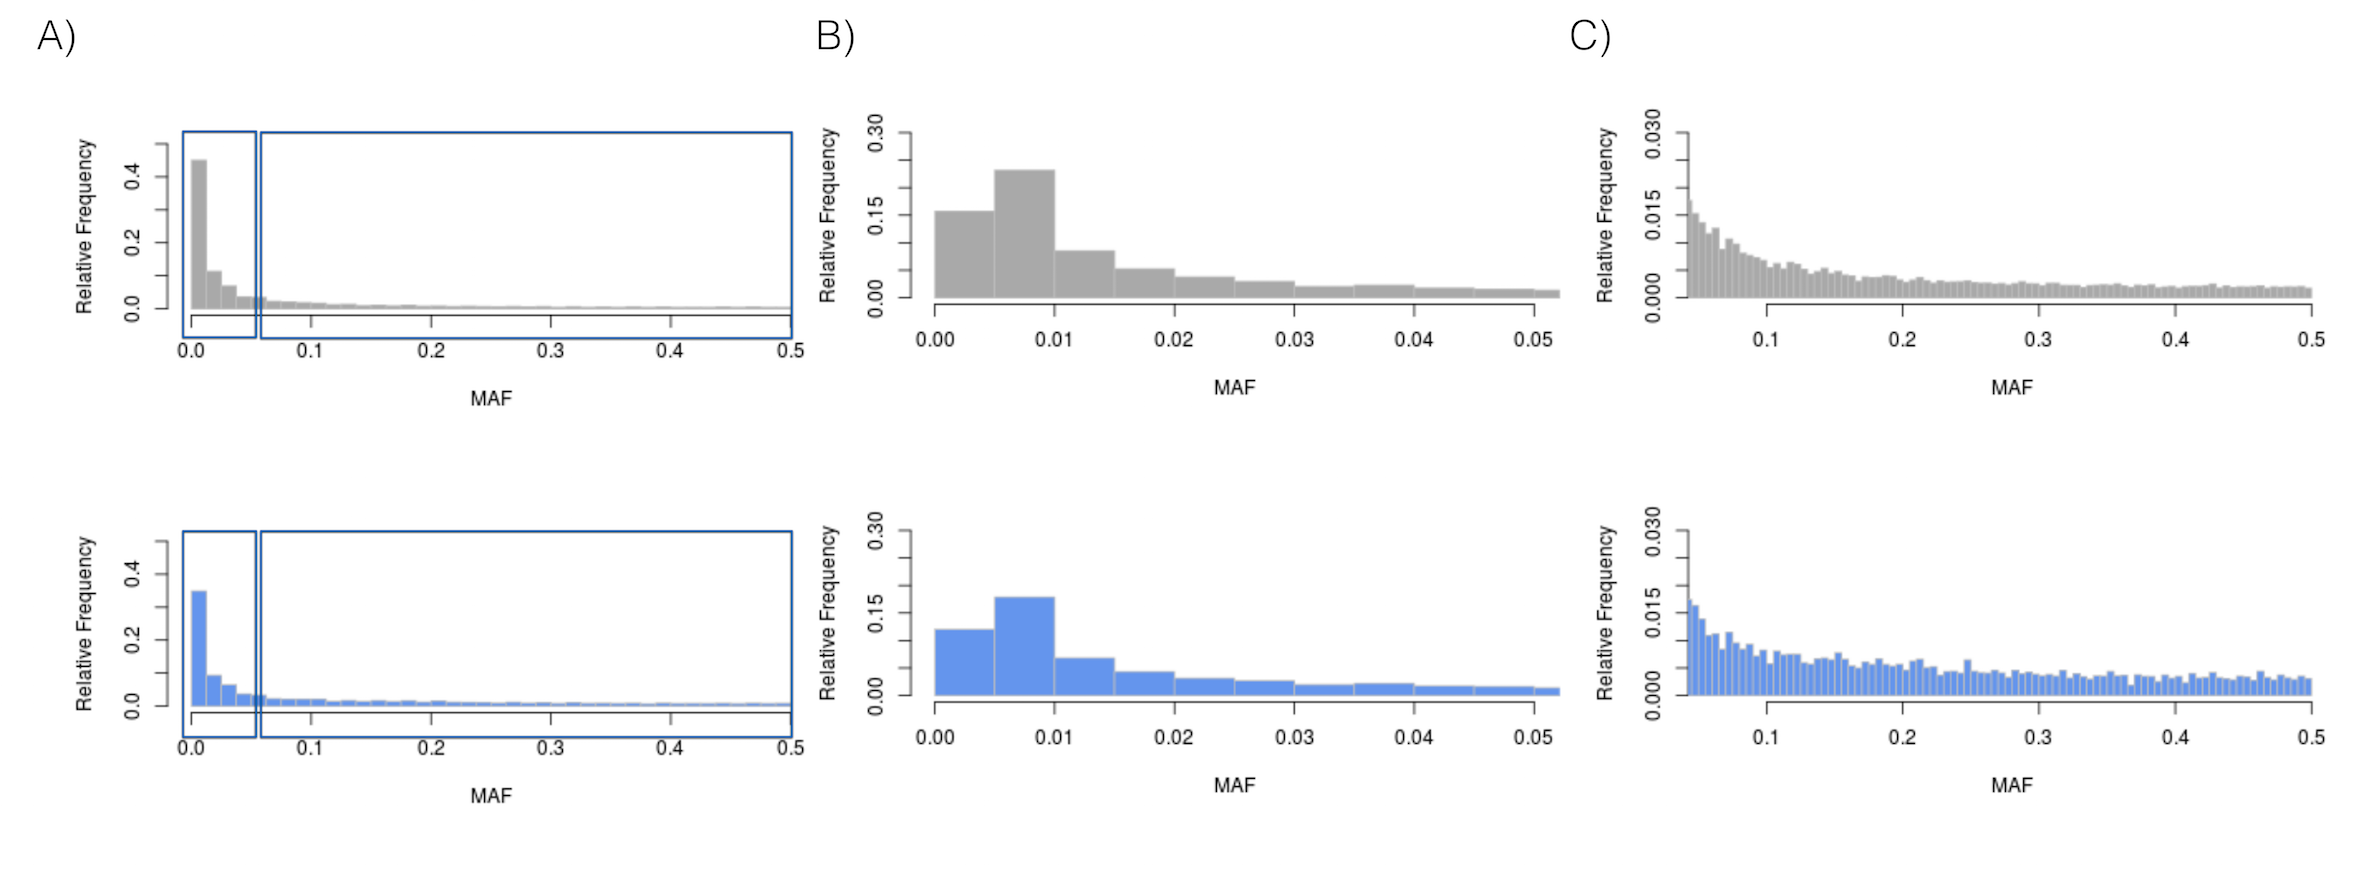
\includegraphics[width= 20 cm, keepaspectratio]
{chap3_folder/figures/SFS_chap2.png}
\caption{\textbf{Site frequency spectrum for protein-coding ($N+S$) SNPs} SNPs come from balanced (blue) and control genes (gray). Rectangles identify the sections that are zoomed in in (B) and (C). } 
\label{fig:SFS}
\end{sidewaysfigure}
%%%%%%%% Figure %%%%%%%%%%%
%%%%%%%% Figure %%%%%%%%%%%

% Para o paper: me ocorreu que o SFS vai ficar mais claro se você plotar ele também usando os log transformed frequencies. Isso irá ressaltar a categoria com efeito forte. 
%BDB: concordo, essa figura tem que melhorar, mas vou deixar assim na tese.

The SFS of the balanced genes is shifted towards intermediate frequencies when compared to the genomic background distribution (Figure ~\ref{fig:SFS}). Specifically, balanced genes have about 10\% less variants in the lower bins of frequency (MAF $\leq 0.0025$). In other words, the balanced genes have a different SFS from that of the background, and an appropriate re-sampling of control SNPs needs to account for this property of the balanced genes. 

The SNPs in the balanced genes were binned according to their MAFs (Table ~\ref{tab:logMAF_bins}), and their distribution into the bins was used for the re-sampling procedure for the controls. Because signatures of LTBS are expected to be restricted to narrow windows (\cite{Andres2009,Andres2011,Bitarello2016,Charlesworth2006}) and here we consider the entire gene, this shift towards intermediate frequencies is modest.

%%%%%%%%%%%%%%%%%%%%%%%%%%%%%%%%%%%%
% this table needs to be completed %
%%%%%%%%%%%%%%%%%%%%%%%%%%%%%%%%%%%%
\begin{sidewaystable}[]
\centering
\scriptsize
\begin{tabular}{@{}ccllclcllllllllllll@{}}
\toprule
\multicolumn{19}{c}{Bins} \\ \midrule
\rowcolor[HTML]{C0C0C0} 
{\color[HTML]{000000} Pop} & \multicolumn{2}{c}{\cellcolor[HTML]{C0C0C0}{\color[HTML]{000000} 1}} & \multicolumn{2}{l}{\cellcolor[HTML]{C0C0C0}2} & \multicolumn{2}{l}{\cellcolor[HTML]{C0C0C0}3} & \multicolumn{2}{c}{\cellcolor[HTML]{C0C0C0}4} & \multicolumn{2}{c}{\cellcolor[HTML]{C0C0C0}5} & \multicolumn{2}{c}{\cellcolor[HTML]{C0C0C0}6} & \multicolumn{2}{l}{\cellcolor[HTML]{C0C0C0}7} & \multicolumn{2}{l}{\cellcolor[HTML]{C0C0C0}8} & \multicolumn{2}{l}{\cellcolor[HTML]{C0C0C0}9} \\ \cmidrule(r){1-19} 
\multicolumn{1}{l}{} & \multicolumn{1}{l}{n} & MAF & n & \multicolumn{1}{l}{MAF} & n & \multicolumn{1}{l}{MAF} & n & MAF & n & MAF & n & MAF & n & MAF & n & MAF & n & MAF \\ \cmidrule(r){2-19}
YRI & 905 & 0.5-0.5 & 277 & 0.9-0.9 & 317 & 1.4-1.8 & 348 & 2.3-3.7 & 292 & 4.2-6.9 & 320 & 7.4-12.5 & 361 & 13-22.2 & 416 &  22.7- 39.3 & 187 & 39.8-50 \\
LWK & 977 & 0.5-0.5 & 386 & 1-1 & 355 & 1.5-2 & 283 & 2.5-3.5 & 335 & 4-7 & 282 & 7.6-12.1 & 390 & 12.6-22.2 & 383 & 22.7-39.4 & 196 & 40-50 \\
MSL & 894 & 0.6-0.6 & 304 & 1.12-1.2 & 208 & 1.8-1.8 & 333 & 2.3-3.5 & 364 & 4.1-7 & 309 & 7.6-12.3 & 390 & 12.9-22.3 & 390 & 22.9-39.4 & 195 & 40-50 \\
GWD & 974 & 0.4-0.4 & 304 & 0.9-0.9 & 395 & 1.3-2.2 & 269 & 2.6-3.5  & 322 & 4-6.6 & 311 & 7.1-12.4 & 368 & 12.8-22.1 & 404 & 22.6-39.4 & 203 & 39.8-50 \\
ESN & 790 & 0.5-0.5 & 303 & 1-1 & 306 & 1.5-2 & 268 & 2.5-3.5 & 334 & 4-7.1 & 300 & 7.6-12.1 & 372 & 12.6-22.2 & 388 & 22.7-39.4 & 200 & 39.9-50 \\
TSI & 820 & 0.5-0.5 & 173 & 0.9-0.9 & 167 & 1.4-1.9 & 175 & 2.3-3.7 & 171 & 4.2-7 & 177 & 7.5-12.1 & 329 & 12.6-22 & 390 & 22.4-39.7 & 194 & 40.2-50 \\
GBR & 586 & 0.55-0.55 & 162 & 1.1-1.1 & 150 & 1.6-2.2 & 145 & 2.7-3.8 & 157 & 4.4-6.6 & 194 & 7.1-12.1 & 313 & 12.6-22 & 363 & 22.5-39.6 & 229 & 40.1-50 \\
FIN & 409 & 0.5-0.5 & 143 & 1-1 & 171 & 1.5-2 & 153 & 2.5-3.5 & 196 & 4-7 & 203 & 7.6-12.1 & 304 & 12.6-22.2 & 370 & 22.7-39.4 & 304 & 39.9-50 \\
CEU & 644 & 0.5-0.5 & 147 & 1-1 & 138 & 1.5-2 & 160 & 2.5-3.5 & 194 & 4-7.1 & 165 & 7.6-12.1 & 325 & 12.6-22.2 & 376 & 22.7-39.4 & 204 & 39.9-50 \\
IBS & 825 & 0.5-0.5 & 173 & 0.9-0.9 & 176 & 1.4-1.8 & 158 & 2.3-3.7 & 191 & 4.2-7 & 176 & 7.5-12.1 & 311 & 12.6-22 & 392 & 22.4-39.7 & 210 & 40.2-50  \\ \bottomrule
\end{tabular}
\caption{\textbf{Binning of SNPs according to their minor allelic frequencies}\\ SNPs in balanced genes were binned according to their logMAF values (see Methods). Values  correspond to the set of balanced genes with HLA SNPs included. When HLA SNPs were excluded, the bin proportions changed (not shown). n, number of SNPs ($N+S$) in the bin; MAF, minimum and maximum MAF values observed within the bin. MAFs are given in \%.}
\label{tab:logMAF_bins}
\end{sidewaystable}

\afterpage{\FloatBarrier}
%%%%%%%%%%%%%%%%%%%%%%%%%%%%%%%%%%%%%%%%%%%%%%%%%%%%%%%%%%%%%%%%%%%%%%%%%%%%%%%%%%%%%
\subsection{Measures of deleteriousness correlate negatively with allelic frequency}
%%%%%%%%%%%%%%%%%%%%%%%%%%%%%%%%%%%%%%%%%%%%%%%%%%%%%%%%%%%%%%%%%%%%%%%%%%%%%%%%%%%%%

Previously, \textcite{Lohmueller2008} reported that SNPs classified as "damaging" according to PolyPhen had significantly lower mean derived allele frequencies (DAF) than "benign" SNPs, with the "probably damaging" category having the lowest mean DAF.

More generally, nonsynonymous variants are expected to have lower frequencies (\cite{Brandvain2016}), because purifying selection will have had enough time to purge deleterious variants from the population (assuming most nonsynonymous variants are deleterious). This is in fact the pattern seen for human populations, where there is a vast excess of low frequency nonsynonymous variants (\cite{Casals2013,Fu2012,Tennessen2012}). Moreover, C scores also tend to be higher for lower frequency variants (\cite{Kircher2014}), although it has been shown that C score distributions have power to differentiate lead-SNPs and tag-SNPs from GWAS, which by definition have similar frequencies (\cite{Kircher2014}).


We confirmed these patterns with the 1000 Genomes data we analyzed (Figure ~\ref{fig:logMAF_bins_2}). When dividing all protein-coding  SNPs (whether they fall into balanced genes or not) into bins of minor allele frequencies (logMAF, see Methods), a clear negative correlation is observed between MAF and the three statistics: $P_{N}/P_{S}$, $P_{del}/P_{S}$ and Cscore (Figure ~\ref{fig:logMAF_bins_2}).

All of the aforementioned observations indicate the importance of controlling for allele frequencies when analyzing the load of deleterious mutations among balanced genes. Lack of a control would cause higher load among control SNPs than for the SNPs from balanced genes, as a consequence of an enrichment in intermediate frequency variants in balanced genes (\cite{Bitarello2016}) and the fact that deleterious variants are more abundant in the lower bins of MAF (\cite{Adzhubei2010,Kircher2014,Lohmueller2008,Subramanian2016}).


%%%%%% Figure %%%%%%% Figure %%%%%%% Figure %%%%%%%%%%%
%%%%%% Figure %%%%%%% Figure %%%%%%% Figure %%%%%%%%%%%
\newpage
\begin{sidewaysfigure}[h]
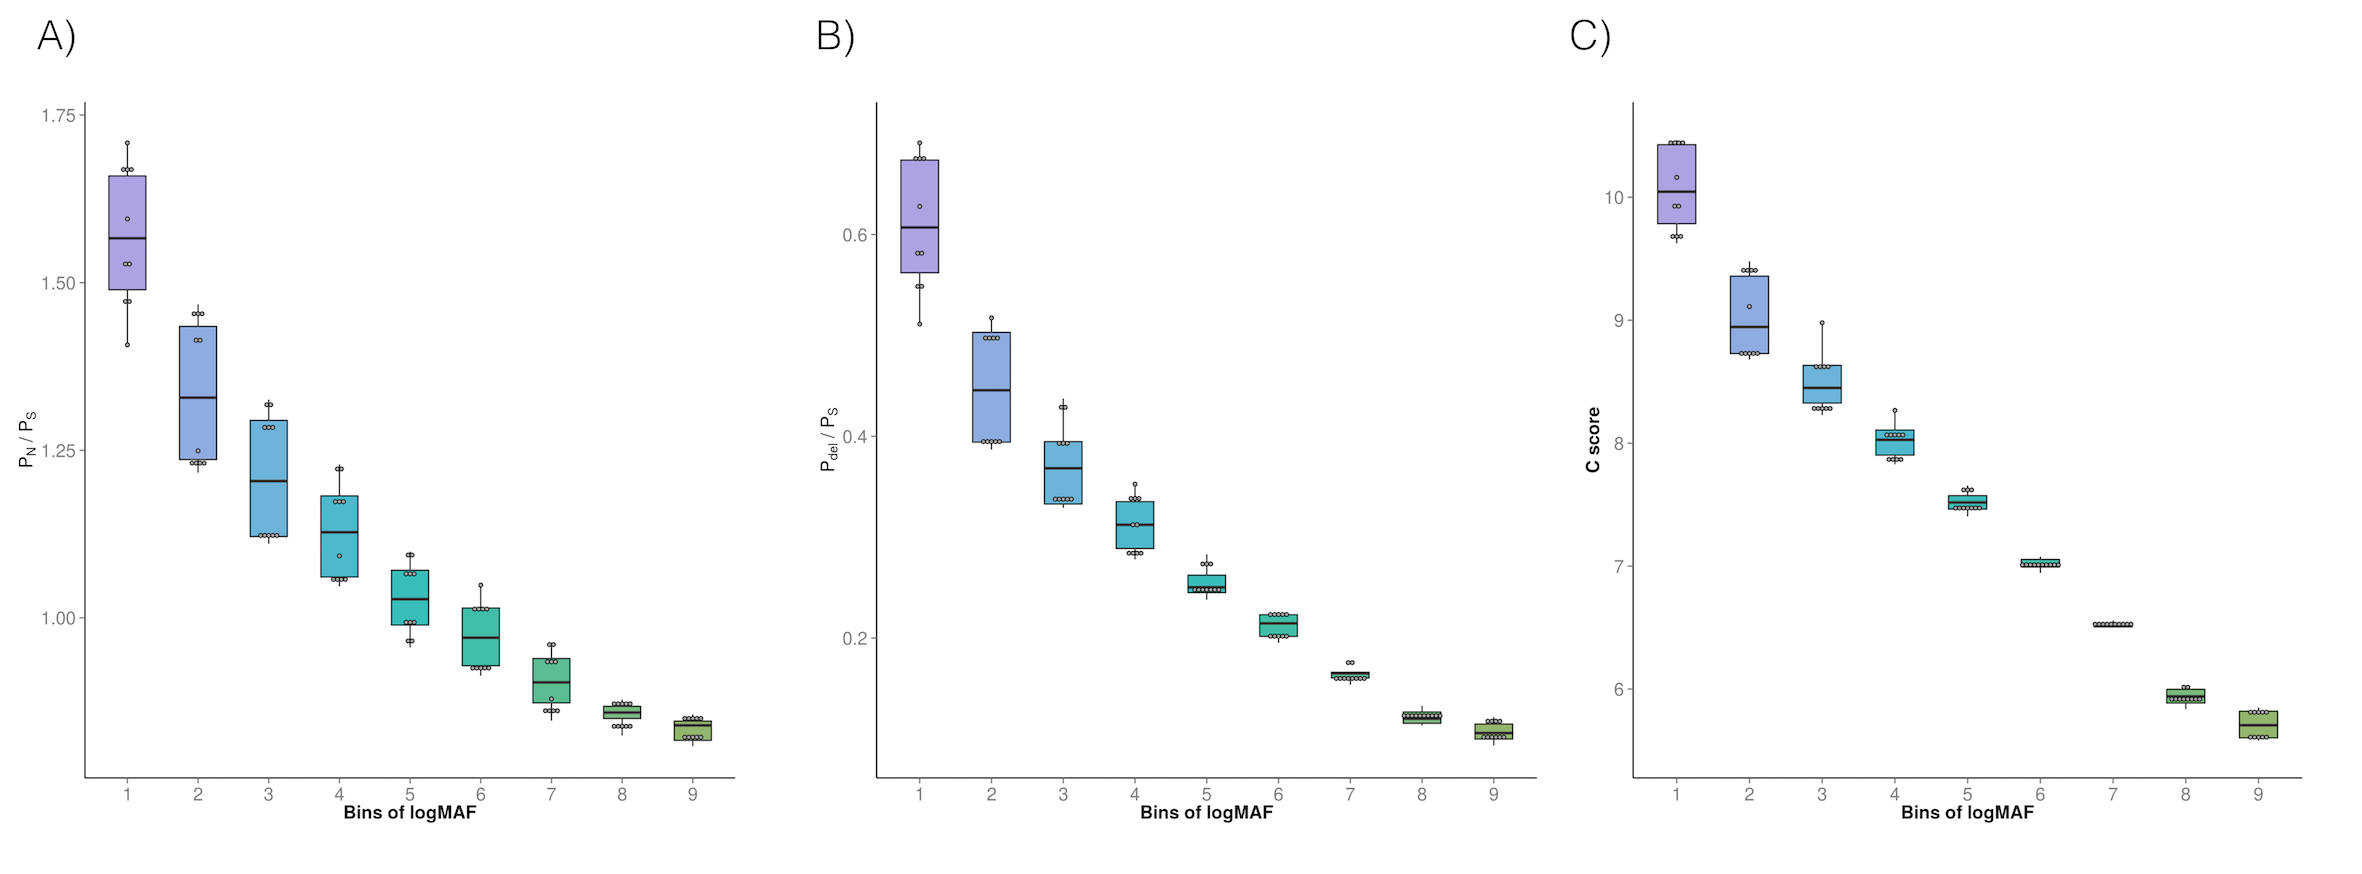
\includegraphics[]{chap3_folder/figures/logMAF_bins_2.png}
\caption{\textbf{Boxplot of load statistics by each bin of MAF.}
All autosomic $N+S$ SNPs were included here. Bins were defined based of the log(base 10) of the MAF of each variant (see Methods).
y-axis, (A) $P_{N}/P_{S}$, (B) $P_{del}/P_{S}$, (C) Cscore.
}
\label{fig:logMAF_bins_2}
\end{sidewaysfigure}

%%% Figure %%%%%%% Figure %%%%
%%% Figure %%%%%%% Figure %%%%



%%% Figure %%%%%%% Figure %%%%
%%% Figure %%%%%%% Figure %%%%
\begin{sidewaysfigure}[h]
\centering
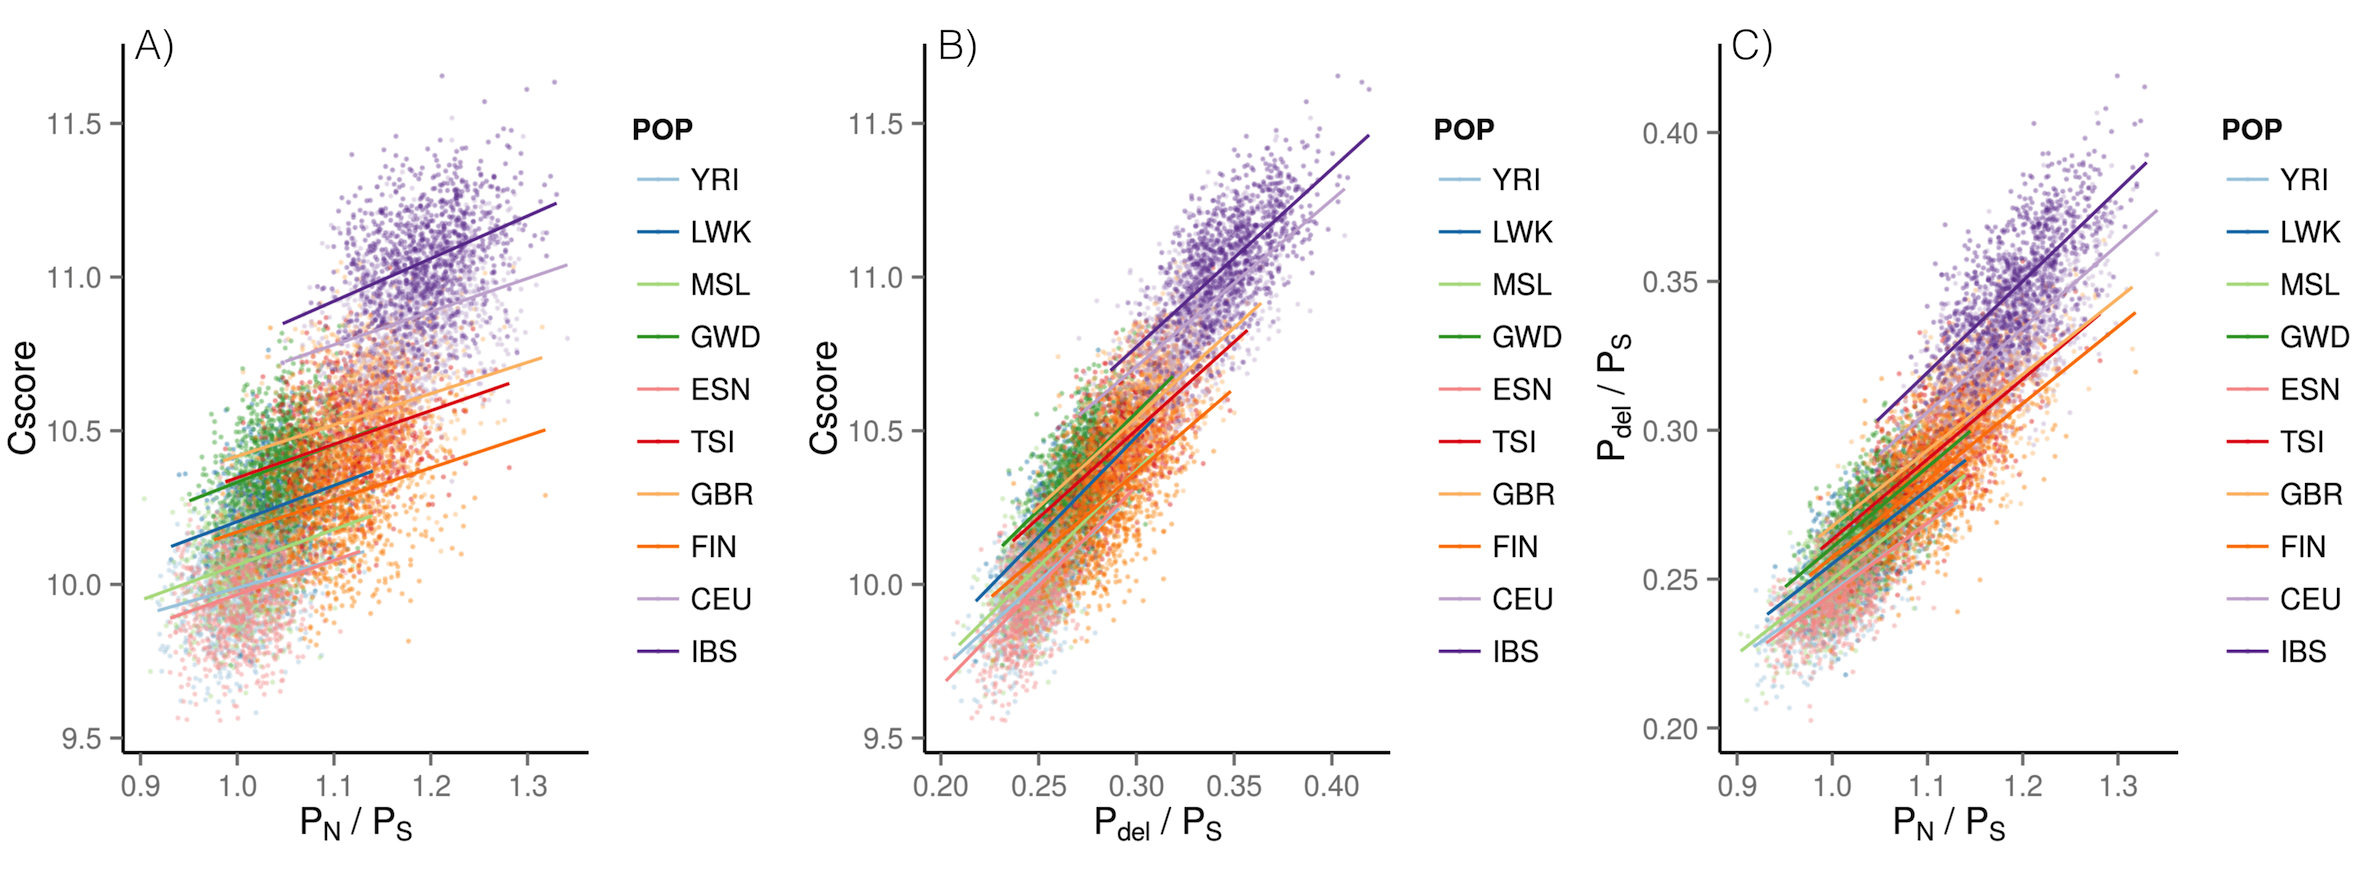
\includegraphics[]{chap3_folder/figures/scatter_del_controls.png}
\caption{\textbf{Correlations between load summary statistics.} (A) C score and $P_{N}/P_{S}$ (cor=0.80, for all populations combined, Pearson, p-value $< 2.2^{e-16}$), (B) $P_{del}/P_{S}$ and Cscore (cor=0.91, $p< 2.2e^{-16}$) and (c) $P_{del}/P_{S}$ and $P_{N}/P_{S}$ (cor=0.91, $p< 2.2e^{-16}$). Each color corresponds to one population and each point is refers to the metric estimated for a re-sampled set of SNPs. Lines represent linear regressions for each population. For correlation values per population, see Table ~\ref{tab:correlations}.}

\label{fig:scatter}
\end{sidewaysfigure}
%%% Figure %%%%%%% Figure %%%%
%%% Figure %%%%%%% Figure %%%%

%%% Table %%% Table %%% Table %%% Table %%% Table %%% Table 
%%% Table %%% Table %%% Table %%% Table %%% Table %%% Table 
%%% Table %%% Table %%% Table %%% Table %%% Table %%% Table 


\begin{table}[h]
\centering
\begin{tabular}{@{}cccc@{}}
\toprule
\rowcolor[HTML]{C0C0C0} 
{\color[HTML]{000000} Pop} & {\color[HTML]{000000} $P_{N}/P_{S}$-Cscore} & {\color[HTML]{000000} $P_{del}/P_{S}$-Cscore} & {\color[HTML]{000000} $P_{N}/P_{S}$-$P_{del}/P_{S}$} \\ \midrule
YRI & 0.23 & 0.55 & 0.61\\
LWK & 0.27 & 0.61 & 0.62 \\
MSL & 0.28 & 0.59 & 0.65 \\
GWD & 0.28 & 0.61 & 0.65 \\
ESN & 0.26 & 0.58 & 0.63 \\
TSI & 0.28 & 0.60 & 0.67 \\
GBR & 0.27 & 0.60 & 0.65 \\
FIN & 0.27 & 0.56 & 0.65 \\
CEU & 0.28 & 0.59 & 0.68 \\
IBS & 0.36 & 0.67 & 0.70 \\ \bottomrule
\end{tabular}
\caption{\textbf{Pearson's correlations between load statistics.} Each value corresponds to 1,000 re-samplings (controls) for the balanced SNPs (gene-based). All correlations are highly significant ($p-value < 2.6e^{-13}$).
}
\label{tab:correlations}
\end{table}
%%%%%%%%%%%%%%%%%%%%%%%%%%%%%%%%%%%%%%%%%%%%%%%
%%%%%%%%%%%%%%%%%%%%%%%%%%%%%%%%%%%%%%%%%%%%%%%


Although our three measures of deleteriousness differ in the criteria used to define/quantify how damaging variants are, we find an overall high correlation among these measures (Figure ~\ref{fig:scatter}). $P_{N}/P_{S}$ and $P_{del}/P_{S}$ are highly correlated in all populations (cor$>0.61$ and $p<2.6e^{-13}$, Table ~\ref{tab:correlations}), and Cscore and $P_{del}/P_{S}$ as well (cor$>0.55$, Table ~\ref{tab:correlations}). $P_{N}/P_{S}$ and Cscore have a weaker correlation, albeit also highly significant (Figure ~\ref{fig:scatter}A and Table ~\ref{tab:correlations}).

These results indicate the importance of using a re-sampling approach that controls for differences in frequencies of SNPs in balanced genes and genomewide (Table ~\ref{tab:logMAF_bins}). Re-sampling sets of genes which are not under balancing selection, without controlling for the SFS, would lead the control to be relatively enriched for low frequency variants, a factor which would obscure the identification of possible differences between the balanced and control SNPs.


\afterpage{\FloatBarrier}
%%%%%%%%%%%%%%%%%%%%%%%%%%%%%%%%%%%%%%%%%%%%%%%%%%%%%%%%%%%%
\afterpage{\clearpage}
\subsection{Extreme values for HLA SNPs} 
%%%%%%%%%%%%%%%%%%%%%%%%%%%%%%%%%%%%%%%%%%%%%%%%%%%%%%%%%%%%

In the scan for balancing selection of \textcite{Bitarello2016}, HLA genes were over-represented among the category of selected genes, and showed extremely strong evidence for selection, with 12 classical HLA genes present among the 213 genes with strongest signatures of balancing selection. This observation, associated to the fact that HLA genes are likely to carry several sites under the direct effects of balancing selection, led us to single them out for an exploratory analysis. %do we need ref for HLA here?

We initially compared the load statistics for the set of SNPs from balanced genes to a group comprising all control SNPs in the genome. Note that here there was no re-sampling involved; we simply compared the statistics between the different groups. We evaluated the influence of SNPs from HLA genes on the load summary statistics by excluding all HLA SNPs from the set of SNPs contained in balanced genes.

The set of SNPs from the balanced genes have different values for the three statistics when compared to the control set of SNPs: $P_{N}/P_{S}$ values are higher (Figure ~\ref{fig:logMAF_bins}), while $P_{del}/P_{S}$ and C score values are lower for the SNPs from all balanced genes (Figure ~\ref{fig:logMAF_bins}). Interestingly, the HLA set of SNPs follows the same pattern as the SNPs from the set of all balanced genes  (which include the HLA SNPs), although in a much stronger way. When we examine HLA genes alone, we find that the average  $P_{N}/P_{S}$ for these loci is almost 2-fold greater than that of control SNPs (Figure ~\ref{fig:logMAF_bins}). Similarly, the reduction in $P_{del}/P_{S}$ and C score in HLA compared to control SNPs is also about two-fold (Figure ~\ref{fig:logMAF_bins}). Moreover, when HLA SNPs are removed from the set of SNPs from balanced genes, the remaining set tends to have values closer to controls, albeit still different (Figure ~\ref{fig:logMAF_bins}).

The extreme patterns of HLA SNPs for these three statistics could be driving the patterns seen in the SNPs from balanced genes, of which they are part of. The $P_{N}/P_{S}$ result is conservative in the sense that, although one could expect lower values for HLA genes (less low frequency and thus less nonsynonymous variants), it is actually almost two-fold higher (Figure ~\ref{fig:logMAF_bins}). This observation likely results from the   high number of sites that are actively maintained by balancing selection in these genes. It is a well-known fact that balancing selection has targeted several sites in HLA genes (e.g. \cite{Hughes1988,Yang2002a,Bitarello2015}), which could at least partially explain the patterns observed for $P_{N}/P_{S}$. The mechanisms driving diversity in the other balanced genes, however, remain largely unknown, and it is reasonable to assume that only one (or a few) site(s) has been targeted by balancing selection in a given gene (e.g. in \cite{Leffler2013a} i.e, that the HLA represents the exception, rather than the rule. 

However, there is no obvious biological explanation as to why $P_{del}/P_{S}$ and C scores should be reduced in HLA compared to control SNPs. This suggests that the reason might be related to allelic frequencies. Moreover, the HLA genes are enriched  not only in intermediate frequency alleles (which are less likely to be deleterious) but also in number of polymorphic sites (\cite{Robinson2013}). Thus, although  HLA genes represent only 12 out of 213 balanced genes considered here, given the high SNP density of the MHC region as a whole, they account for a considerable proportion of the SNPs from balanced genes (Table ~\ref{tab:balancedSNPs}). Thus, in the remaining analyses we estimated load for the set of SNPs from balanced genes with and without the inclusion of HLA SNPs. Because the HLA SNPs change the shape of the SFS, we also re-sampled the control SNPs accordingly.


%%%%%% Figure %%%%%%% Figure %%%%%%% Figure %%%%%%%%%%%
%%%%%% Figure %%%%%%% Figure %%%%%%% Figure %%%%%%%%%%%

\begin{sidewaysfigure}[h]
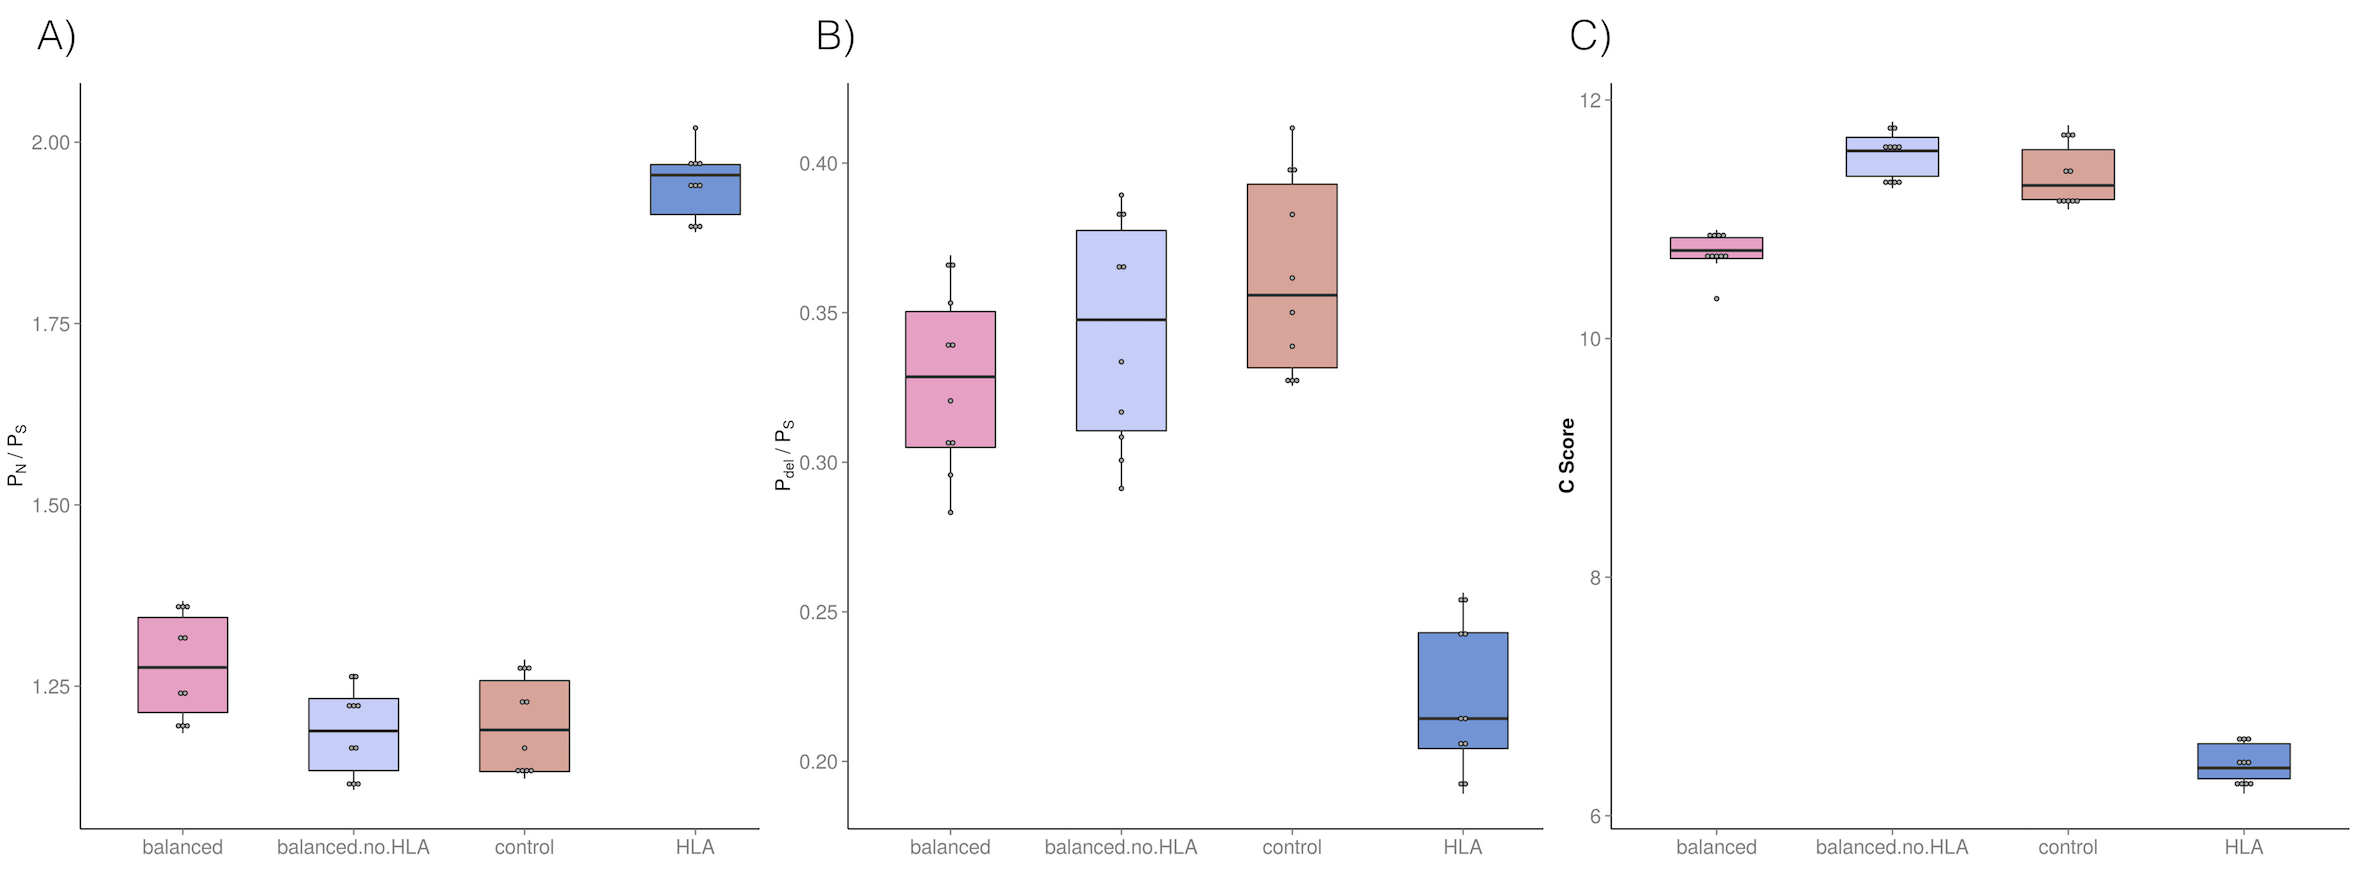
\includegraphics[]{chap3_folder/figures/logMAF_bins.png}
\caption{\textbf{Boxplot of load statistics sets of SNPs.}
Balanced, SNPs contained in the balanced genes; balanced.no.HLA, same as the previous category, but excluding 12 HLA genes (see Methods); control, all SNPs not contained in balanced genes; HLA, a set of 12 HLA genes (see Methods). Each boxplot is composed of 10 data points, each one corresponding to a population (see Methods). y-axis, (A) $P_{N}/P_{S}$, (B) $P_{del}/P_{s}$, (C) Cscore.
}
\label{fig:logMAF_bins}
\end{sidewaysfigure}
%

\afterpage{\FloatBarrier}
%%%%%%%%%%%%%%%%%%%%%%%%%%%%%%%%%%%%%%%%%%%%%%%%%%%%%%%%%%%%%%%%%%%%%%%%%%%%%%%%%%%
\subsection{Increased nonsynonymous to synonymous SNPs in balanced genes}  
%%%%%%%%%%%%%%%%%%%%%%%%%%%%%%%%%%%%%%%%%%%%%%%%%%%%%%%%%%%%%%%%%%%%%%%%%%%%%%%%%%%
Firstly, we note that $P_{N}/P_{S}$ values are on average higher for European than for African populations (Figure ~\ref{fig:PnPs_combo}). This confirms the finding that European populations have a higher proportion of nonsynonymous variants than African populations (\cite{Lohmueller2008}). Since our re-sampling was done by population, we intrinsically take this into account as seen in the control distributions (Figure ~\ref{fig:PnPs_combo}).

The $P_{N}/P_{S}$ values of SNPs from balanced genes are significantly higher than controls ($p<0.01$; Figure ~\ref{fig:PnPs_combo}A). These results are not explained by the HLA genes: although their removal reduces the balanced $P_{N}/P_{S}$ (as expected), while slightly increasing the control values (because the target SFS changes, thus resulting in less intermediate frequencies in the controls), the increase in of balanced genes with respect to the controls remains significant, albeit less extreme (Figure ~\ref{fig:PnPs_combo}B, $P<0.01$ for all African populations and GBR and FIN). One European population has marginally significant values ($P=0.06$, TSI) and for two others (CEU and IBS) $P_{N}/P_{S}$ falls within the control distribution after the removal of HLA SNPs ($P>0.24$, Figure ~\ref{fig:PnPs_combo}B).

The increased $P_{N}/P_{S}$ for balanced genes is also not likely driven by the putative target(s) of balancing selection in these genes: when $P_{N}/P_{S}$ for the balanced genes was estimated after removing the SNP(s) with the highest heterozygosity(ies) for each gene (see Methods), results remain qualitatively similar (Figure ~\ref{fig:PnPs_combo}). In fact, most of the SNPs excluded from the balanced genes were intronic ($\sim 90$\% for all populations, Table ~\ref{tab:Hremove}), and on average 11.5 \emph{N} and 14.6 \emph{S} SNPs were removed from each population (Table ~\ref{tab:Hremove}) which makes the $P_{N}/P_{S}$ estimates increase slightly in most cases (Figure ~\ref{fig:PnPs_combo}). 

These results suggest there is an excess of nonsynonymous variants within the set of balanced genes, and that this excess, at least for African populations, is not entirely explained by the presence of HLA genes (Figure ~\ref{fig:PnPs_combo}B) nor by the presence of a one or a few SNPs per gene that have very high heterozigosities (and are presumably the actual targets of selection). For the European populations the removal of HLA SNPs decreased the estimates in relation to controls in a more pronounced way.

Because nonsynonymous variants are not necessarily deleterious (they might also be neutral), we also investigated two other measures of load that directly quantify deleteriousness.

%%%%%% Figure %%%%%%% Figure %%%%%%% Figure %%%%%%%%%%%
%%%%%% Figure %%%%%%% Figure %%%%%%% Figure %%%%%%%%%%%
\begin{sidewaysfigure}[h]
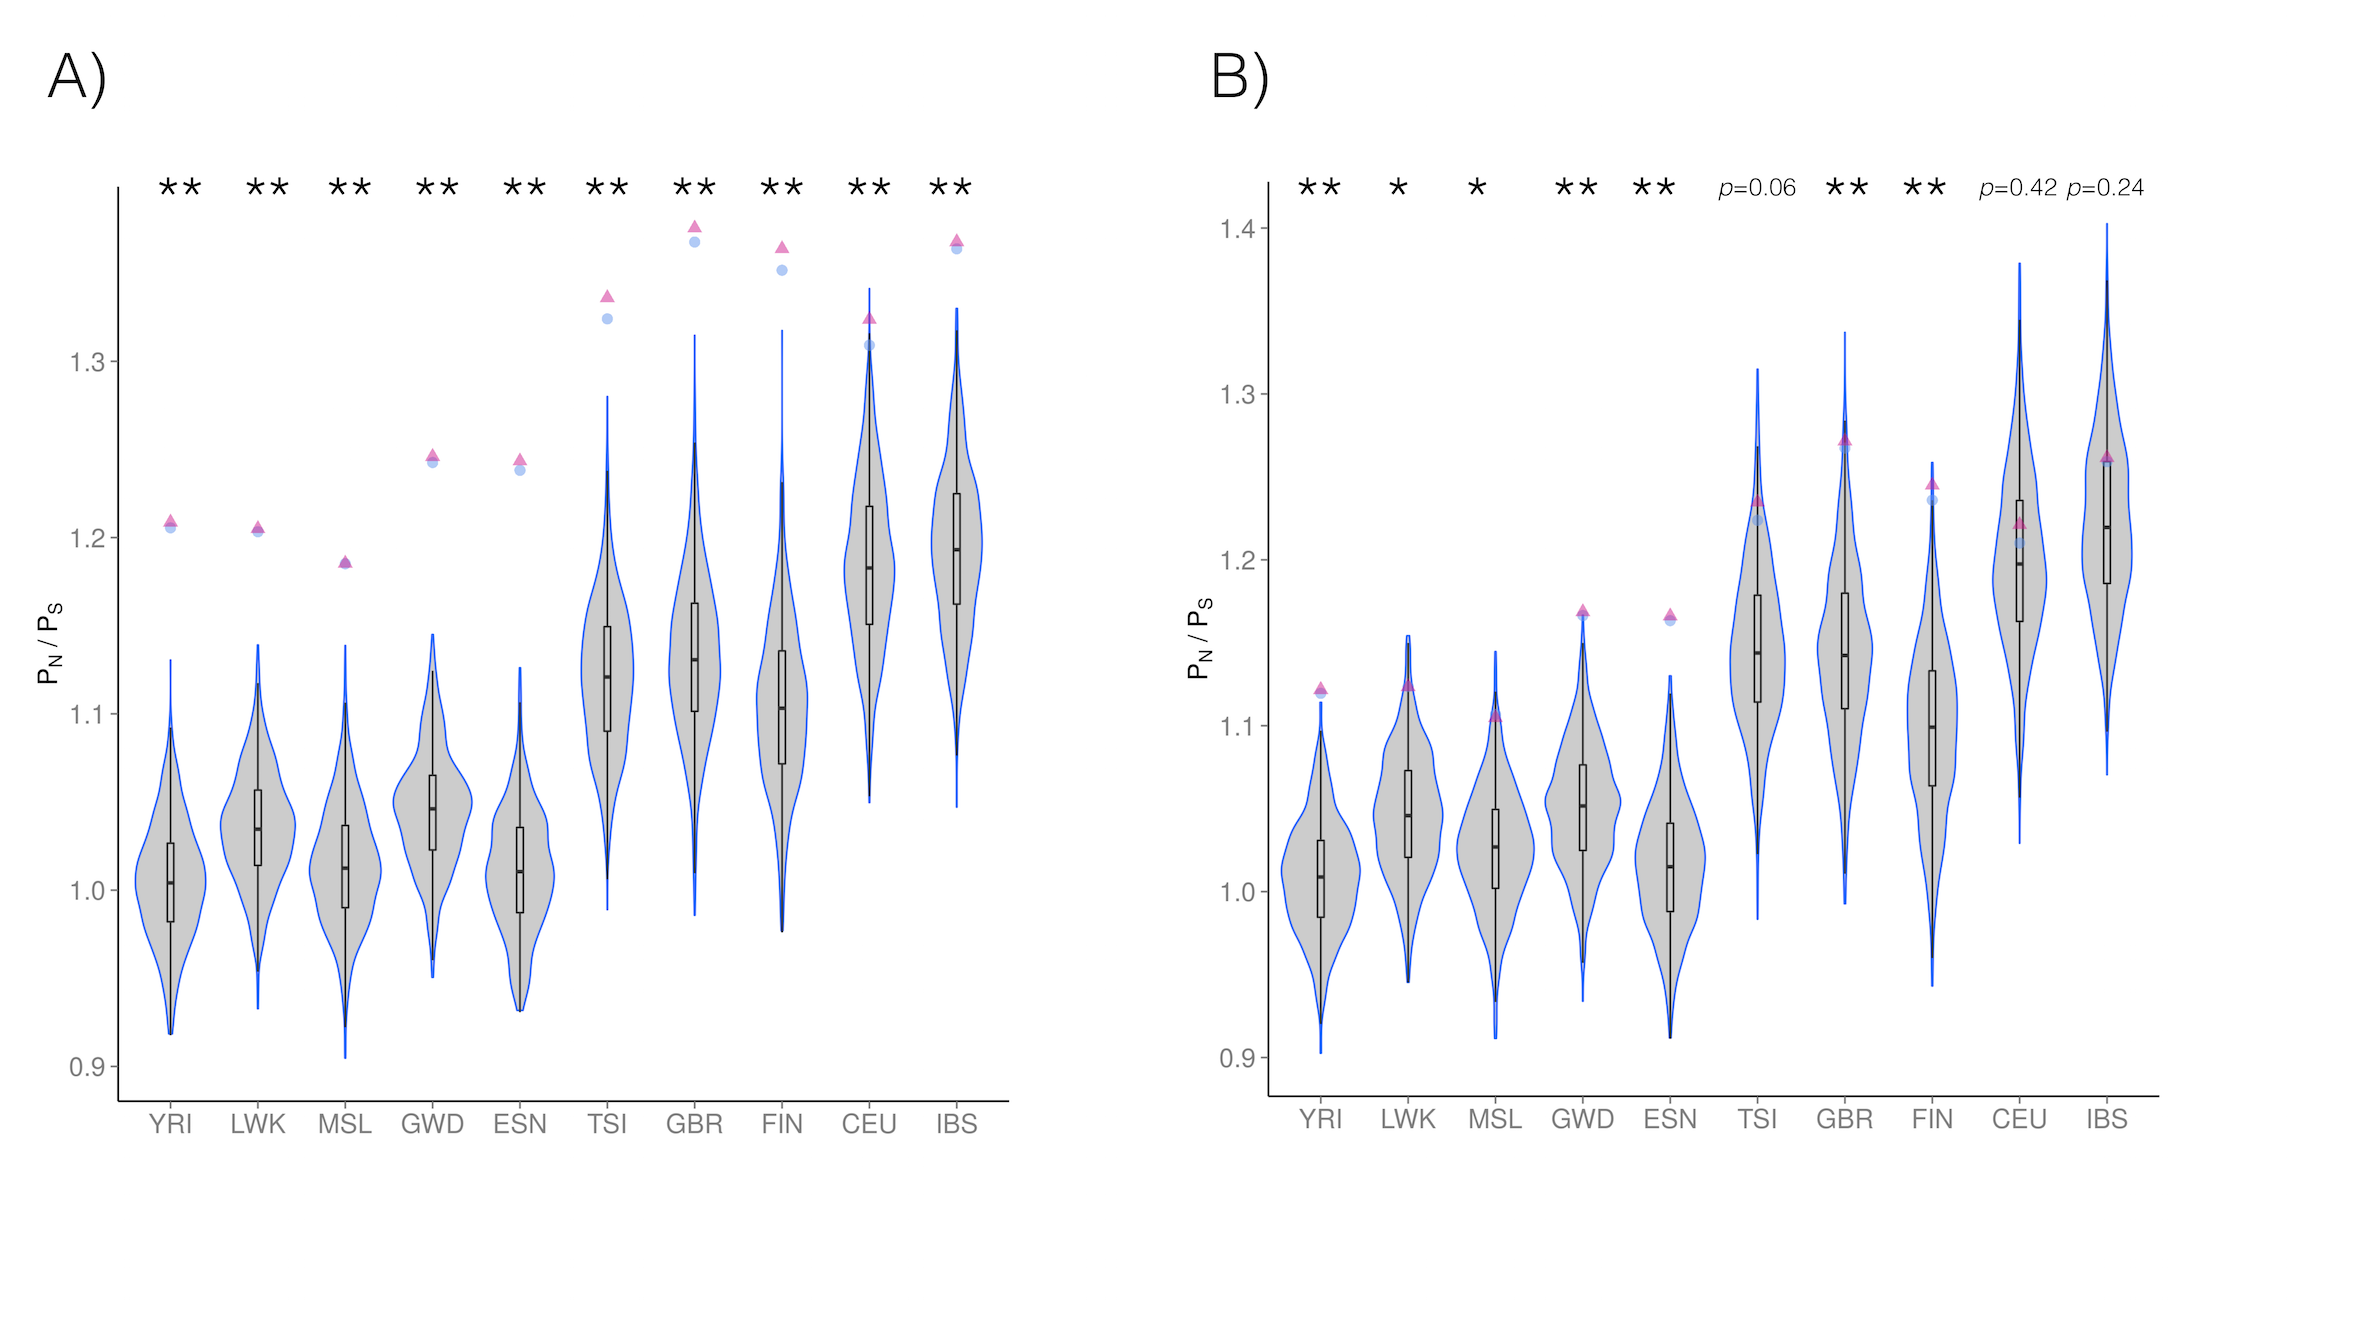
\includegraphics[]{chap3_folder/figures/PnPs_combo2.png}
\caption{\textbf{$P_{N}/P_{S}$ for balanced genes} A) Including HLA SNPs; B) removing HLA SNPs. Blue circle, estimate for all protein-coding SNPs in the set; pink triangle, estimate after removal of SNP(s) with highest heterozygosity in each gene (see Methods. **, $p-value<0.01$, *$p<0.05$. Reported p-values are for the estimates with all SNPs.}
\label{fig:PnPs_combo}
\end{sidewaysfigure}

%%%%%% Figure %%%%%%% Figure %%%%%%% Figure %%%%%%%%%%%
%%%%%% Figure %%%%%%% Figure %%%%%%% Figure %%%%%%%%%%%
%%%%%%%%%%%%%%%%%%%%%%%%%%%%%%%%%%%%%%%%%%%%%%%%%%%%%%%

%%%%%%%%%%%%%%%%%%%%%%%%%%%%%%%%%%%%%%%%%%%%%%%%%%%%%%%%%%%%%%%%%%%%%%%%%%%%%%%%%%%%%%%%%%%%%%%%%%%%%%%%%%%%%%%%%%%%%%
\subsection{Increased proportion of damaging to synonymous SNPs in balanced genes} 
%%%%%%%%%%%%%%%%%%%%%%%%%%%%%%%%%%%%%%%%%%%%%%%%%%%%%%%%%%%%%%%%%%%%%%%%%%%%%%%%%%%%%%%%%%%%%%%%%%%%%%%%%%%%%%%%%%%%%%

Again, we note that European populations have higher balanced and control values than African populations, as seen previously (\cite{Lohmueller2008}). When comparing $P_{del}/P_{S}$ estimates for SNPs from balanced genes and control sets of SNPs, a similar pattern emerges, although less extreme than the one seen for $P_{N}/P_{S}$: balanced genes tend to have higher load compared to controls ($p<0.05$) for all populations, except CEU and IBS ($p>0.14$; Figure ~\ref{fig:PdelPs_combo}A).


The removal of HLA SNPs only slightly changes the $P_{del}/P_{S}$, and the qualitative relationship between them does not change, with all populations except CEU and IBS having $p<0.05$ (Figure ~\ref{fig:PdelPs_combo}). This differs from what was observed for $PN/PS$, where the removal of HLA SNPs made the estimates of load for balanced genes less different from controls, although still highly significant. 

Moreover, the $P_{del}/P_{S}$ estimates with and without the removal of SNPs with the highest heterozygosity per gene  only slightly increase the estimates, compatible with the observation that few of the removed SNPs with this filter are nonsynonymous, and always less than the number of synonymous SNPs (Table ~\ref{tab:Hremove}).

The results for $P_{del}/P_{S}$ are in agreement with what was observed for $P_{N}/P_{S}$, suggesting that the patterns observed for $P_{N}/P_{S}$ are driven by deleterious, and not adaptive or neutral nonsynonymous variants. 

%%%%%% Figure %%%%%%% Figure %%%%%%% Figure %%%%%%%%%%%
%%%%%% Figure %%%%%%% Figure %%%%%%% Figure %%%%%%%%%%%

\begin{sidewaysfigure}[h]
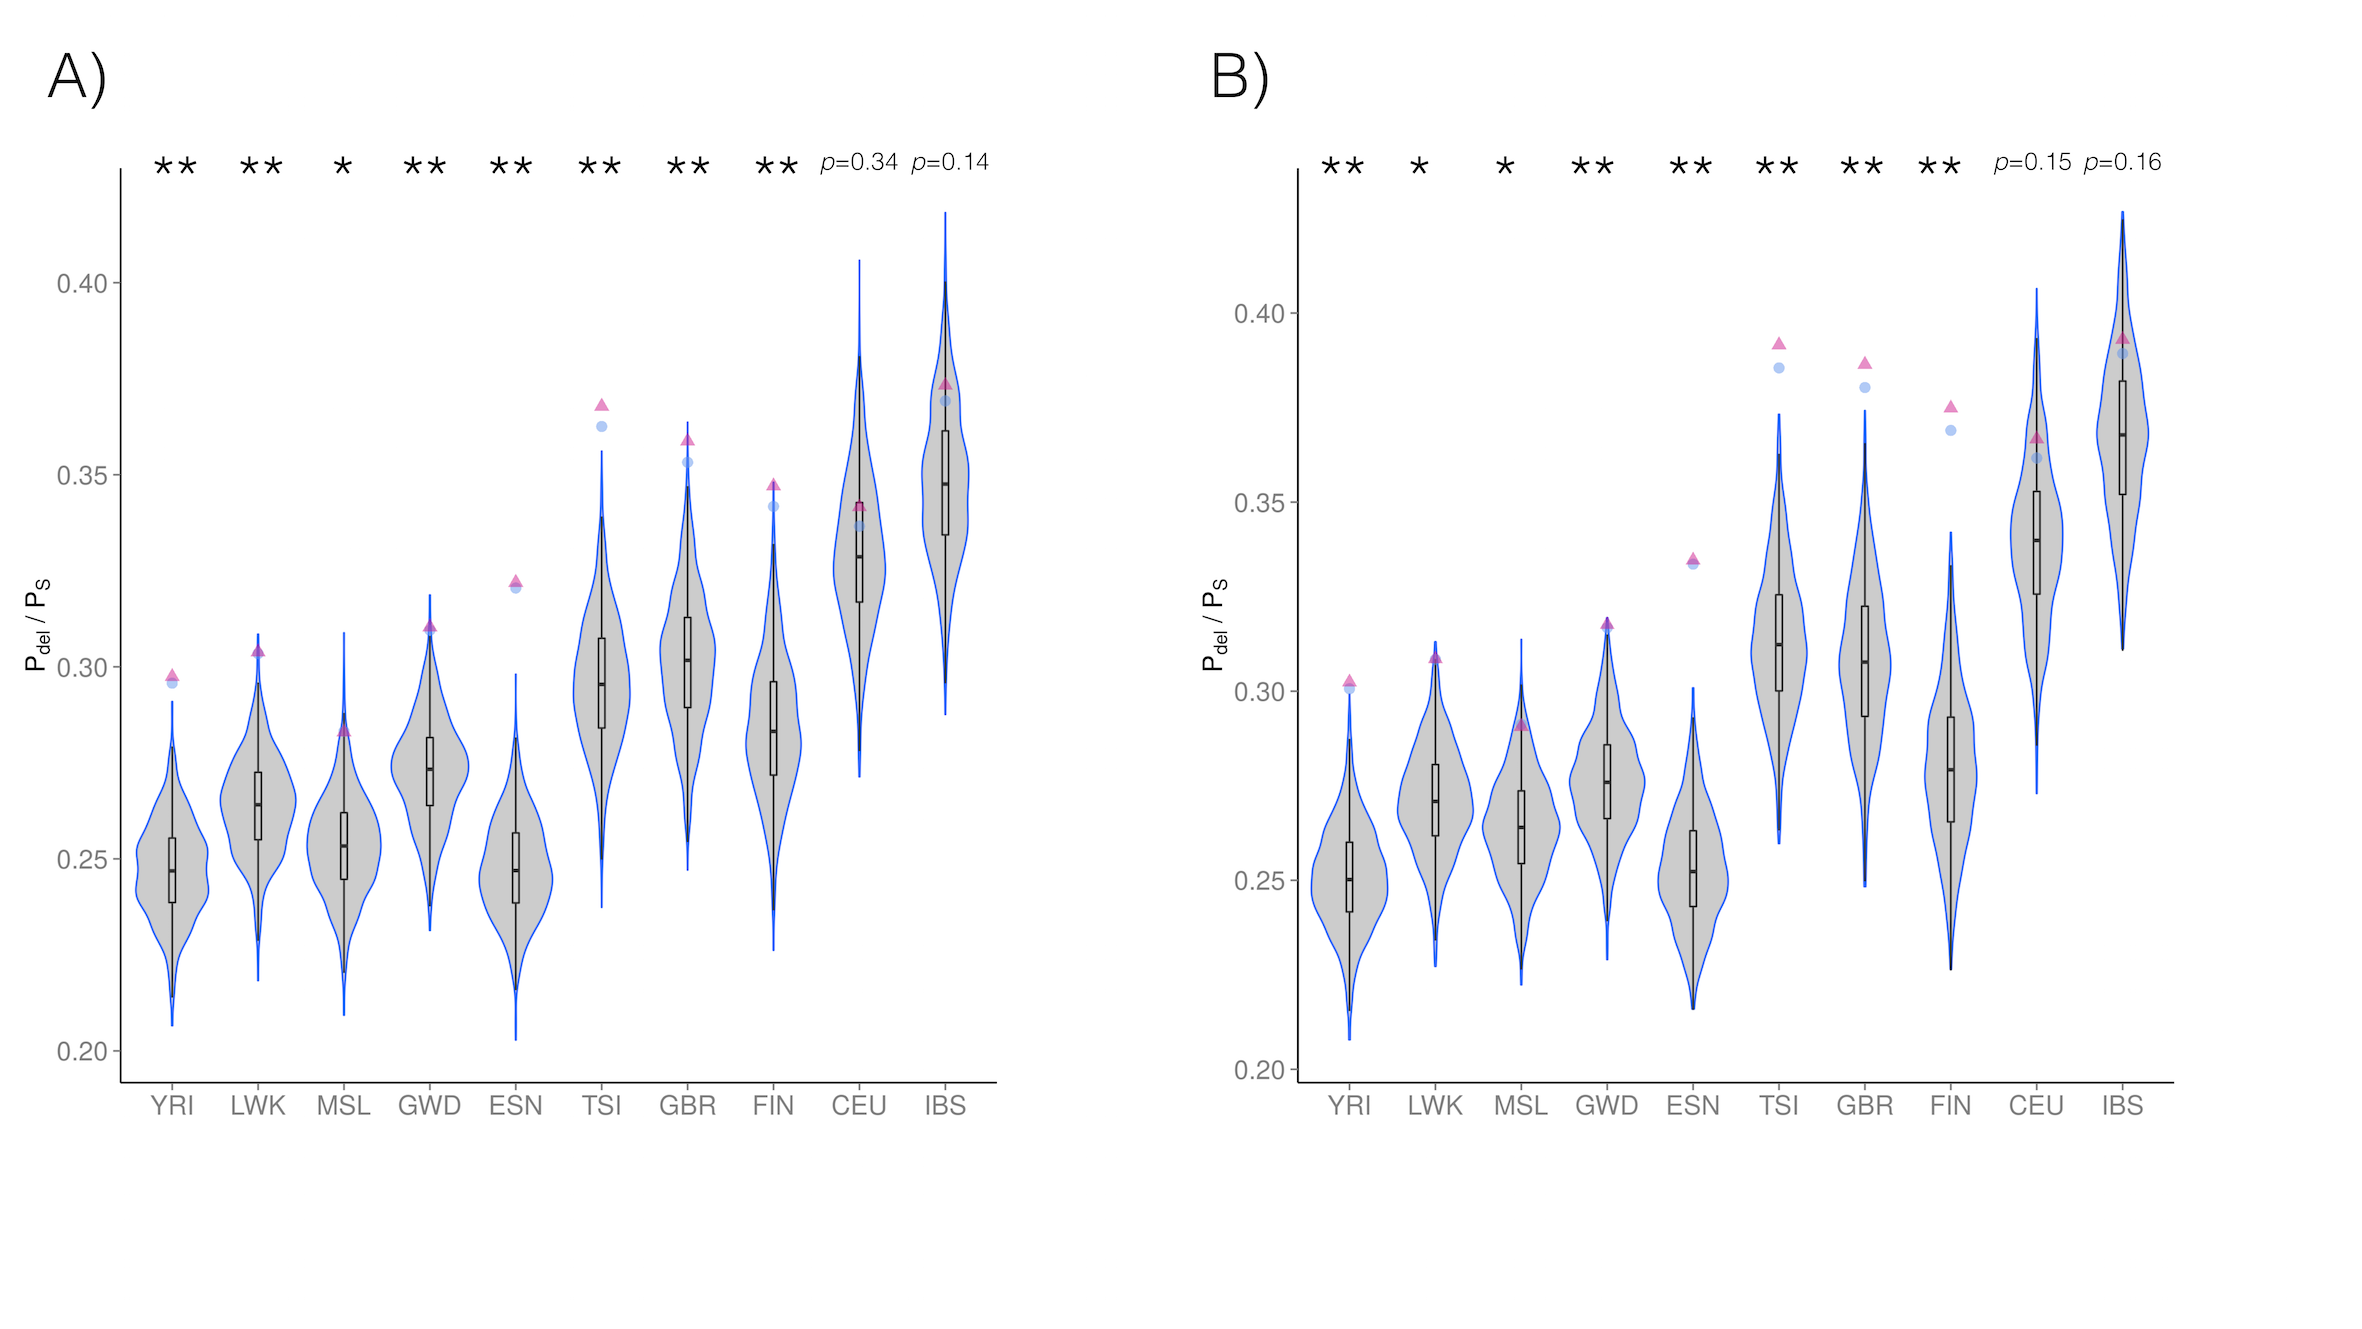
\includegraphics[]{chap3_folder/figures/PdelPs_combo2.png}
\caption{\textbf{$P_{del}/P_{S}$ for balanced genes} A) Including HLA SNPs; B) removing HLA SNPs. Blue circle, estimate for all protein-coding SNPs in the set; pink triangle, estimate after removal of SNP(s) with highest heterozygosity in each gene (see Methods). **, $p<0.01$, *$p<0.05$. Reported p-values are for the estimates with all SNPs.}
\label{fig:PdelPs_combo}
\end{sidewaysfigure}

%%%%%% Figure %%%%%%% Figure %%%%%%% Figure %%%%%%%%%%%
%%%%%% Figure %%%%%%% Figure %%%%%%% Figure %%%%%%%%%%%

\afterpage{\FloatBarrier}
%%%%%%%%%%%%%%%%%%%%%%%%%%%%%%%%%%%%%%%%%%%%%%%%%%%%%%%%%%%%%%%%%%%%%%%%
%%%%%%%%%%%%%%%%%%%%%%%%%%%%%%%%%%%%%%%%%%%%%%%%%%%%%%%%%%%%%%%%%%%%%%%%
\subsection{Increased C-scores in balanced genes} 

Average scaled C scores yield qualitatively different results with respect to analyses based on $P_{N}/P_{S}$ and $P_{del}/P_{S}$. Firstly, for African populations and for TSI the load estimates for balanced genes are very elevated ($p<0.01$) compared to controls, similarly to what was seen for $P_{N}/P_{S}$ (Figure ~\ref{fig:Cscore_combo}A). However, this pattern is not observed for the other European populations, with p-values approaching one for CEU and IBS (Figure ~\ref{fig:Cscore_combo}A). Interestingly, in this case, the removal of HLA SNPs enhances the signal: African values become even more extreme and all the European populations acquire extreme values when compared to controls as well ($p<0.01$ for all populations, Figure ~\ref{fig:Cscore_combo}B).


%%%%%% Figure %%%%%%% Figure %%%%%%% Figure %%%%%%%%%%%
%%%%%% Figure %%%%%%% Figure %%%%%%% Figure %%%%%%%%%%%
\begin{sidewaysfigure}[h]
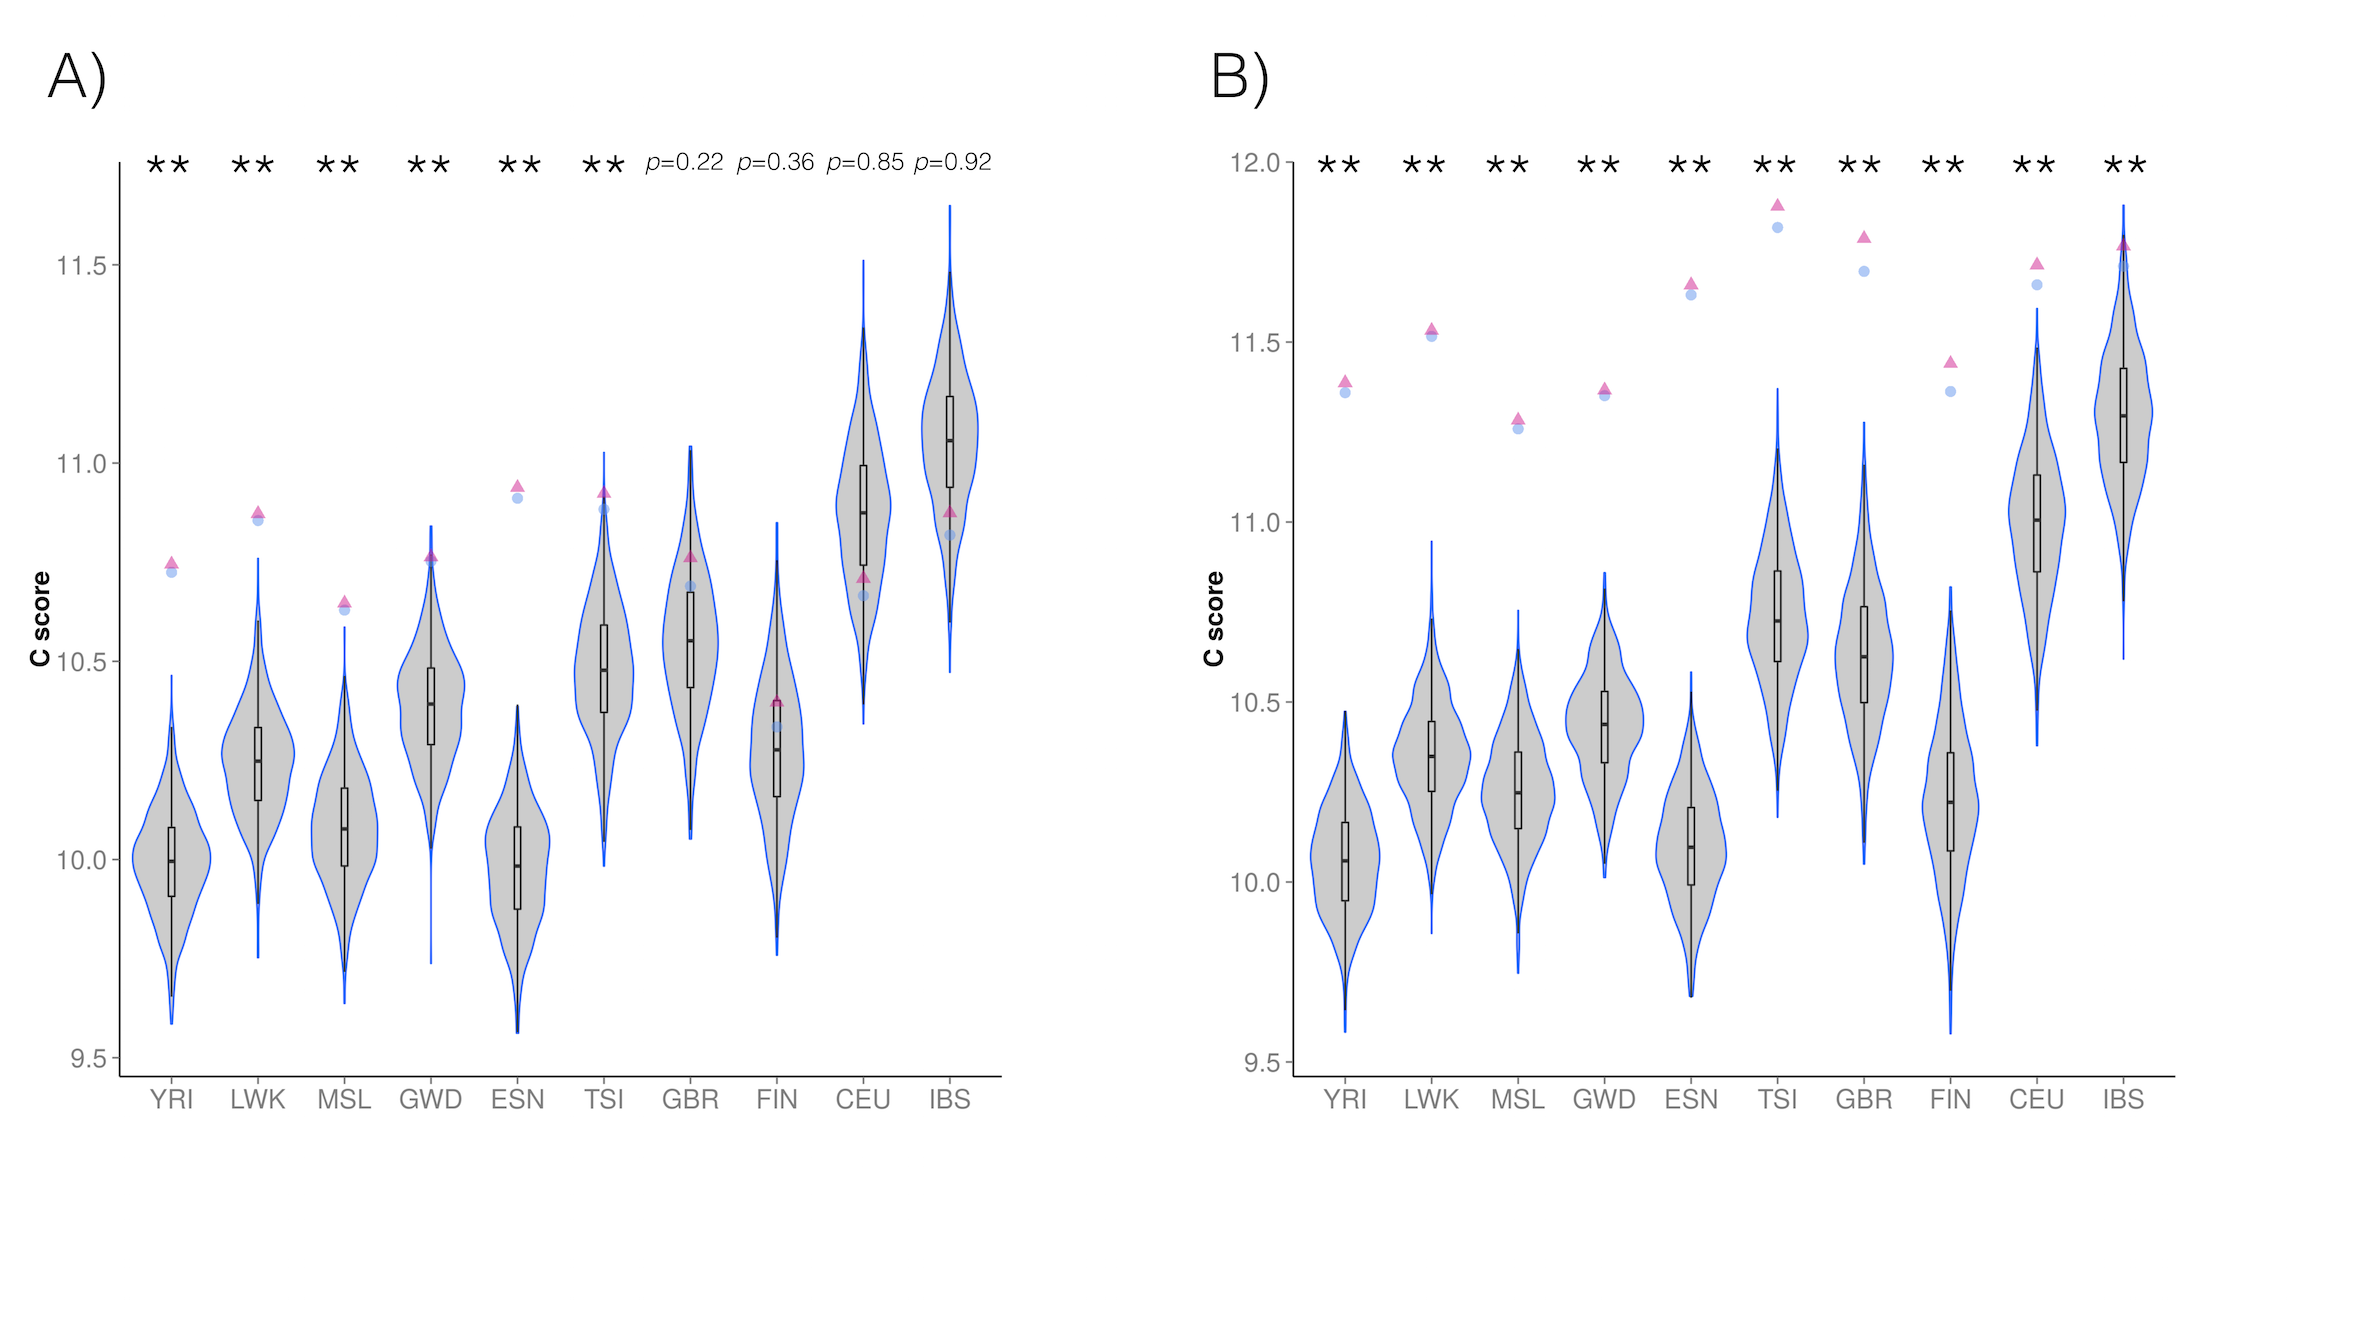
\includegraphics[]{chap3_folder/figures/Cscore_combo2.png}
\caption{\textbf{Average scaled Cscore for balanced genes.} A) Including HLA SNPs; B) removing HLA SNPs. Blue circle, estimate for all protein-coding SNPs in the set; pink triangle, estimate after removal of SNP(s) with highest heterozygosity in each gene (see Methods). **, $p<0.01$, *$p<0.05$. Reported p-values are for the estimates with all SNPs.}
\label{fig:Cscore_combo}
\end{sidewaysfigure}

%%%%%% Figure %%%%%%% Figure %%%%%%% Figure %%%%%%%%%%%
%%%%%% Figure %%%%%%% Figure %%%%%%% Figure %%%%%%%%%%%


Given that the most appropriate set of SNPs for testing our hypothesis of load  is the set without HLA genes and without the SNPs with the highest heterozigosities per gene (Figure ~\ref{fig:Cscore_combo}B), pink triangle), it is plausible that the reduction or loss of significance of the load in the set of all balanced genes (in Africa and Europe, respectively) is due to the excess of adaptive variants (from HLA or other genes) present in the complete set, which tend to have lower C scores. Note that the control distributions in Figures ~\ref{fig:Cscore_combo}A and ~\ref{fig:Cscore_combo}B are very similar, and what changes dramatically is the load estimate for the balanced genes. Also, the Scaled C scores are PHRED-scaled, ranging from 1 to 99, with the top 10\% most deleterious variants having scores above 10, and the top 1\% above 20, and so on (\cite{Kircher2014}). Thus this difference is likely to be even greater than what is conveyed by this analysis.


We also looked at the raw C scores which provide more power in tests comparing sets of SNPs (\cite{Kircher2014}). For African populations, balanced genes have raw C score distributions with significantly higher values than the controls (Mann-Whitney U test, one-tailed, P<=0.05) for more than 70\% of the control re-samplings (Table ~\ref{tab:rawC}), except for GWD, for which only 251 out of 1,000 controls  have significantly lower C scores than the balanced genes. For Europe, only TSI has 13\% of the controls with lower C scores than the balanced genes, and all other populations have less than 5 such cases (Table ~\ref{tab:rawC}). 

%%%%%%%%% table %%%%%%% table %%%%%%%%%
%%%%%%%%% table %%%%%%% table %%%%%%%%%
\begin{table}[h]
\centering
\begin{tabular}{@{}ccc@{}}
\toprule
\rowcolor[HTML]{C0C0C0} 
{\color[HTML]{000000} Pop} & {\color[HTML]{000000} HLA included} & HLA excluded \\ \midrule
 & $P<0.05$ & \multicolumn{1}{c}{$P<0.05$} \\
YRI & 959 &  1,000 \\
LWK & 805 &  1,000 \\
MSL & 727 &  1,000 \\
GWD & 251 &  1,000 \\
ESN & 995 &  1,000 \\
TSI & 130 &  999 \\
GBR & 5 &  995 \\
FIN & 1 &  999 \\
CEU & 0 & 844 \\
IBS & 0 &  1,000\\ \bottomrule
\end{tabular}
\caption{\textbf{Raw C score comparison between balanced genes and controls}
For each comparison, the alternative hypothesis was that balanced genes had higher raw C score values than the control distribution (Mann-Whitney U test, one-tailed). Values refer to the number of comparisons (out of 1,000 control distributions) for which the null hypothesis (distributions are not different) was rejected ($P<0.05$).
}
\label{tab:rawC}
\end{table}
%%%%%%%%% table %%%%%%% table %%%%%%%%%
%%%%%%%%% table %%%%%%% table %%%%%%%%%

However, when we perform the same analyses for the balanced genes after the removal of HLA SNPs, balanced genes have higher raw C scores for all comparisons in African populations, and for more than 995 comparisons for all European populations, except CEU, for which 844 comparisons are significant (Table ~\ref{tab:rawC}).


%%%%%%%%%%%%%%%%%%%%%%%%%%%%%%%%%%%%%%%%%%%%%%%%%%%%%%%%%%%%%%%%%%%%%%%%%%%%%%%%%%%%%%%%%%%%%%%%%%%%%%%%%%%%%%%%%%%%%%%%%%%%%%%%%%%%%%%%%%%%%%%%
%%%%%%%%%%%%%%%%%%%%%%%%%%%%%%%%%%%%%%%%%%%%%%%%%%%%%%%%%%%%%%%%%%%%%%%%%%%%%%%%%%%%%%%%%%%%%%%%%%%%%%%%%%%%%%%%%%%%%%%%%%%%%%%%%%%%%%%%%%%%%%%%
%%%%%%%%%%%%%%%%%%%%%%%%%%%%%%%%%%%%%%%%%%%%%%%%%%%%%%%%%%%%

\section{Discussion and Conclusions}   %%%%%%%%%%%%%%%%%%%%%
%%%%%%%%%%%%%%%%%%%%%%%%%%%%%%%%%%%%%%%%%%%%%%%%%%%%%%%%%%%%

\subsection{Increased genetic load in balanced genes}

The study of slightly deleterious mutations is one of the pillars of population genetics (\cite{Kondrashov1995}). The fate of mutations is highly dependent on   the effective population size ($N_{e}$) and its relationship to the selection coefficients. As a consequence, weakly deleterious mutations might  reach moderate frequencies in small, but not in large populations, where selection is more effective. Moreover, linkage to selected variants is also a major determinant of the fate of a deleterious mutation (\cite{Hill1966,Cutter2013}).

The fates of strongly deleterious mutations are mostly deterministic in terms of mutation rates and selection coefficients -- i.e, when $s>>1/2N_{e}$ (where $s$ is the selection coefficient). The  fate of very slightly deleterious mutations -- i.e, almost neutral -- is, however, mostly stochastic, driven by genetic drift (\cite{Kondrashov1995}). But what happens when considerably strong selection (positive, negative, balancing) on a site impacts the sites in its vicinity? Here, we examined how balancing selection shapes the accumulation of deleterious mutations in the vicinity of its targets. 

We showed that genes with strong signatures of long-term balancing selection have increased levels of nonsynonymous to synonymous polymorphisms, damaging to synonymous polymorphisms, and also elevated deleteriousness scores (\cite{Kircher2014}), when compared to controls. We took special care in controlling for the fact that balanced genes have a site-frequency spectrum which is different from the genomic background, with proportionally more intermediate frequency variants, and we also accounted for the fact that within the balanced genes there are sites directly under balancing selection, which could be incorrectly assigned to deleterious variants according to some classification methods.

Because HLA genes are known as an example of multi-locus balancing selection -- i.e, several positions within the HLA genes have been targets of selection (\cite{Hughes1988,Yang2002a,Bitarello2015}) -- it seemed plausible that their considerable contribution to the set of balanced genes could be responsible for the overall patterns we observed. Therefore, in all analyses we compared results for balanced genes including and excluding HLA genes. This approach is  conservative, given that not all SNPs in HLA genes are expected to be direct targets of selection. A less drastic solution would be to single out the exons of HLA genes which harbour most -- if not all -- of the balanced polymorphisms in those genes and exclude only the SNPs contained in those exons (\cite{Klein1986}). 

Additionally, we also  removed from each balanced gene the SNP(s) likely to be the targets of balancing selection, in order to filter our datasets from the potentially conflicting patterns generated by advantageous and deleterious variants within the balanced genes. Importantly, in this approach we only excluded the SNP(s) with the highest heterozigosiy among those contained in a window with a very strong signature of LTBS as reported in \textcite{Bitarello2016}, thus increasing the chance that the actual selected site was filtered out.

%%%%%%%%%%%%%%%%%%%%%%%%%%%%%%%%%%%%%%%%%%%%%%%%%%%%%%%%%%%%%%%%%%%%
\subsection{The challenges of quantifying genetic load} 
%%%%%%%%%%%%%%%%%%%%%%%%%%%%%%%%%%%%%%%%%%%%%%%%%%%%%%%%%%%%%%%%%%%%

Establishing the damaging potential of a variant is a formidable task in itself (\cite{Grimm2015}). Quantifying the genetic load and comparing it between groups (populations, SNPs, genes, etc) is also challenging, as demonstrated by the great number of published contrasting results regarding genetic load in humans (reviewed in \cite{Henn2015a}). Therefore, it is important to justify the methodology used here. 

We chose to use statistics based on the counts of deleterious variants ($P_{N}/P_{S}$ and $P_{del}/P_{S}$) and deleteriousness scores (C score). With $P_{N}/P_{S}$ and $P_{del}/P_{S}$ we quantified the proportions of nonsynonymous and potentially damaging variants, respectively, for balanced genes and control groups. $P_{N}$ simply documents whether the  polymorphism changes the coded aminoacid, and thus is unbiased with respect to knowledge of the frequency at which the polymorphism is segregating. Nevertheless, $P_{N}$ counts are composed of neutral, deleterious and advantageous variants and thus are not  straight-forward to interpret. $P_{del}$ is more accurate than $P_{N}$ as a measure of deleteriousness, but it is restricted to  nonsynonymous sites and is only available for a subset of the nonsynonymous variants ($\sim 80$\% for the genome, but $\sim 70$\% for balanced genes), thus reducing its power, particularly in small sets of SNPs. Moreover, PolyPhen-2 has been shown to overfit its training data and not to generalize well for other datasets (\cite{Grimm2015}). Neither of these approaches incorporate the frequency of the deleterious mutations when classifying SNPs.  

One possible frequency-based measure would be the ratio of heterozygosities at nonsynonymous and synonymous sites ( $\pi_{N}/\pi_{S}$ ), but this ratio is particularly sensitive to recent bottlenecks (reviewed in \cite{Brandvain2016}). This is because, after a bottleneck, nonsynonymous variation recovers more quickly than synonymous variation (because there are more nonsynonymous sites), and so an elevated $\pi_{N}/\pi_{S}$  following a bottleneck could be inferred (wrongly) as relaxed  selection. \textcite{Do2015,Simons2014} use and recommend a direct estimate of the number of deleterious (or nonsynonymous) mutations (e.g. $PN/PS$ and $Pdel/PS$), which is robust to violations of demographic equilibrium (reviewed in \cite{Brandvain2016,Henn2015a}). 

Our approach here is thus conservative. Previous studies have shown that for comparisons between African and Out-of-Africa, small or no difference is verified when the number of putative deleterious mutations is counted (\cite{Henn2016,Tennessen2012,Do2015,Lohmueller2014}), whereas on average the out-of-Africa populations are more homozygous for the putative deleterious mutations (\cite{Lohmueller2008}) -- a difference not detectable by these two methods.

In addition to this \enquote{SNP counting} approach, we also compared the distribution of deleteriousness among all SNPs within the balanced genes and controls via the C score (\cite{Kircher2014}) analyses. The C score is defined for all $N+S$ sites and combines desirable features from other annotations, but is also negatively correlated with allelic frequency (as are the other two statistics used here). The C score does not suffer from poor generalization properties like PolyPhen-2, because the vector machine was trained on an independent dataset (\cite{Grimm2015,Kircher2014}). However, CADD (C score) was trained on high frequency variants, and although the C scores are available for all 1000 Genomes Phase 3 variants (\cite{Kircher2014}) its accuracy in differentiating deleteriousness of for low MAF variants is likely to be  smaller.

%%%%%%%%%%%%%%%%%%%%%%%%%%%%%%%%%%%%%%%%%%%%%%%%
\subsection{Sheltered load and hitch-hiking}
%%%%%%%%%%%%%%%%%%%%%%%%%%%%%%%%%%%%%%%%%%%%%%%%
Our observations of increased load in genes with signatures of long-term balancing selection can be explained by two possible mechanisms: 1) as a manifestation of a "sheltered load" (\cite{VanOosterhout2009}) and 2) as an effect of linkage of deleterious variants to the balanced polymorphisms, i.e, a hitch-hiking effect (\cite{Mendes2013,Lenz2016}). 

According to the sheltered load model, regions with an excess of heterozygosity would "protect" rare recessive variants from being "seen" by purifying selection, thus contributing to their permanence in the population and at higher frequencies than expected if they were not linked to balanced polymorphisms. This model has been invoked to explain the dynamics of deleterious mutations near the \emph{S} loci of \emph{Arabidopsis} and \emph{Solanum} (\cite{Stone2004,Roux2013}) and the excess of disease associations in the MHC region (e.g. \cite{VanOosterhout2009}).

On the other hand, recent work (\cite{Lenz2016}) showed through simulations  that deleterious mutations are expected to accumulate in the vicinity of a locus under balancing selection. The simulation framework assumed that several sites were under balancing selection in an HLA-like gene -- as is the case for classic HLA genes (e.g. \cite{Hughes1988,Yang2002a,Bitarello2015}).
% Eu achei que a info de ser HLA like poderia vir depois, mas reverta caso discorde.


Moreover, the simulations assumed symmetrical overdominance and used realistic parameters from the actual HLA genes and/or human demography, such as effective population size, mutation and recombination rates, and even average selection coefficients for these loci. Finally, loci around the selected HLA-like locus were modelled to be either evolving neutrally or under purifying selection. With these simulations, the authors demonstrated that such a scenario leads to an overall reduction of diversity around the HLA-like locus, but the variants that "survive" tend to segregate at higher frequencies, demonstrating the potential for balancing selection in HLA genes to increase the frequency of deleterious variants around the HLA loci. \textcite{Lenz2016} confirm this prediction with empirical data an excess of damaging (\cite{Adzhubei2010}) variants in non-HLA loci of the MHC region. 

Importantly, the simulations of \textcite{Lenz2016} assume an additive model, not a recessive one. Thus, their observations suggest that some other mechanism other than the "sheltered load" is responsible for the increased load in the vicinity of HLA genes, and this is likely to be the hitch-hiking effect mentioned above.  

%%%%%%%%%%%%%%%%%%%%%%%%%%%%%%%%%%%%%%%%%%%%%%%%%%%%%%%%%
%%%%%%%%%%%%%%%%%%%%%%%%%%%%%%%%%%%%%%%%%%%%%%%%%%%%%%%%%
\renewcommand*{\bibfont}{\footnotesize}
\renewcommand\bibname{References} 

\printbibliography[heading=bibintoc]   

%%%%%%%%%%%%%%%%%%%%%%%%%%%%%%%%%%%%%%%%%%%%%%%%%%%%%%%%%
%%%%%%%%%%%%%%%%%%%%%%%%%%%%%%%%%%%%%%%%%%%%%%%%%%%%%%%%%

\end{otherlanguage}
\end{refsection}
